% Bemærk ændret til at passe til processanalysen!!!

\documentclass[a4paper,11pt]{report}    % report tilføjer chapter
\usepackage{fourier}                    % Font
\usepackage[utf8]{inputenc}             % Encoding
\usepackage[danish]{babel}              % Dansk sprog
\usepackage{a4}                         % A4 format
\usepackage[margin=3.0cm]{geometry}     % Til at sætte margin
\usepackage{fancyhdr}                   % pæn header og footer
\usepackage{lastpage}                   % til at finde sidste side
\usepackage{hyperref}                   % Referencer i PDF dokumentet og referencer til labels
\usepackage{float}                      % Til at sætte figurer korrekt
\usepackage{url}                        % Til at lave URL
\usepackage[final,danish]{fixme}        % Fixme final/draft
\usepackage{titlesec}                   % Til at ændre på størrelsen på sections
\usepackage{xr}                         % Gør det muligt at cross referere i andre filer
\usepackage{amsmath}                    % Matematik-ting
\usepackage{mathtools}                  % Flere matematik-ting
\usepackage{multirow}                   % Multirows i tabel
\usepackage{threeparttable}             % Til fodnoter i tabeller
\usepackage{listingsutf8}               % Til sourcecode highlight i utf8 format
\usepackage{natbib}                     % Udvidelse af kilder
\usepackage[toc,page]{appendix}         % Til bilag
\usepackage{enumitem}

\let\tnote\relax                        % Fjerner ctable konflikt men ødelægger potientielt noget andet

\usepackage{graphicx}                   % Billeder
\usepackage{pdfpages}                   % PDF sider
\usepackage{color}                      % Farver

% Dokument informationer
\newcommand{\gruppen}{B2-24}
\newcommand{\rapportnavn}{Automatisér dit hjem - Procesanalyse}
\newcommand{\currentpage}{\thepage}     % nuværende side
\newcommand{\numpages}{\pageref{LastPage}}% antal sider
\newcommand{\sidetal}{Side {\currentpage} af {\numpages}} % side informationer
\newcommand{\pagetitle}{\rightmark}     % nuværende sektion
\newcommand{\gruppenummer}{B2-24}
\newcommand{\figuregroup}{(Figuren er fremstillet af gruppen)}
\newcommand{\tabelgroup}{(Tabellen er fremstillet af gruppen)}
\newcommand{\authjem}{Automatiseret hjem}

% Definerer titel osv.
\title{\rapportnavn}
\author{\gruppen}
\date{December 2013}

% Setup af header og footer
\fancypagestyle{plain}{                 % plain er standard for kapitler
    \fancyhead[RO]{Automatisér dit hjem}
    \fancyhead[LO]{Procesanalyse}
    \fancyfoot[CO]{\sidetal}
}
\pagestyle{plain}

% Fjerner afstand mellem kapitel og sætter størrelsen på skriften - se evt. her: http://tex.stackexchange.com/questions/63390/how-to-decrease-spacing-before-chapter-title
\titleformat{\chapter}[display]{\normalfont\huge\bfseries}{\chaptertitlename\ \thechapter}{20pt}{\Huge}
\titlespacing*{\chapter}{0pt}{0pt}{20pt}

% Skriftstørrelse på sections
\titleformat*{\section}{\LARGE\bfseries}
\titleformat*{\subsection}{\Large\bfseries}
\titleformat*{\subsubsection}{\large\bfseries}
\titleformat*{\paragraph}{\normalsize\bfseries}
\titleformat*{\subparagraph}{\normalsize\bfseries}

% Opretter subsubsubsection og subsubsubsubsection
\newcommand{\subsubsubsection}[1]{\paragraph{#1}\mbox{}\\}
\newcommand{\subsubsubsubsection}[1]{\subparagraph{#1}\mbox{}\\}

% Definerer antallet af overskrifter der har tal, samt antallet af overskrifter i indholdsfortegnelsen
\setcounter{secnumdepth}{1}             % 5 Fix for paragraph er en overskrift
\setcounter{tocdepth}{1}                % 5 Fix for paragraph er i indholdsfortegnelse

% Indent til og fra
\newcommand{\enableIndent}{\setlength\parindent{3pt}}
\newcommand{\disableIndent}{\setlength\parindent{0pt}}
\disableIndent

\hyphenation{}                         % Orddeling

% Ændrer indstillingerne for caption for figurer, tabeller og kodestykker - tilføjer bla. kusiv og gør typenavnet bold (eks. Figur 1.1: bliver fed)
\usepackage[font=small,format=plain,labelfont=bf,up,textfont=it,up]{caption}

% Danske bogstaver i kodefiler
\lstset{literate=%
    {æ}{{\ae}}1
    {å}{{\aa}}1
    {ø}{{\o}}1
    {Æ}{{\AE}}1
    {Å}{{\AA}}1
    {Ø}{{\O}}1
}

% Source code farve
\definecolor{gray95}{gray}{.95}

% Source code
\lstdefinestyle{sourceC}
{ 
	numbers=left,
	numbersep=5pt,
	stepnumber=1,
	captionpos=b,
	keywordstyle=\color[rgb]{0,0,1},
	commentstyle=\color[rgb]{0.133,0.545,0.133},
	stringstyle=\color[rgb]{0.627,0.126,0.941},
	backgroundcolor=\color{gray95},
	frame=lrtb,
	framerule=0.5pt,
	linewidth=1.00\textwidth,
	tabsize=4,
	numberbychapter=true,
	basicstyle=\ttfamily\footnotesize,
	language=C,
	breaklines=true,
	showstringspaces=false,
	breakindent=20pt
}

% Source code tekster
\renewcommand{\lstlistingname}{Kode}
\renewcommand{\lstlistlistingname}{Koder}

% Kildeliste
\bibpunct[, ]{[}{]}{;}{n}{,}{,} 		% Definerer de 6 parametre ved Harvard henvisning (bl.a. parantestype og seperatortegn)
%\bibliographystyle{Bibtex/Vancouver}    % Udseende af litteraturlisten
\bibliographystyle{unsrtnat} %plainnat}            % Inkluderer bl.a. isbn numre

% Oprettelse af links inde i pdf dokumentet
\hypersetup{
    pdftitle={\rapportnavn},
    pdfauthor={\gruppen},
    pdfsubject={\rapportnavn},
    bookmarksnumbered=true,
    bookmarksopen=false,
    bookmarksopenlevel=1,
    colorlinks=false,
    pdfstartview=Fit,
    pdfpagemode=UseOutlines,
    pdfpagelayout=TwoPageRight,
    pdfborder = {0 0 0}
}

\hbadness=10001          % Slår alle underfull badness warnings fra
\hfuzz=5.002pt           % Slår de ligegyldige overfull warnings fra

% FixMe
% http://mirrors.dotsrc.org/ctan/macros/latex/contrib/fixme/fixme.pdf
\newcommand{\fix}[1]{\fxnote{#1}}
\newcommand{\dfix}[1]{\fxfatal{#1}}
\renewcommand\fxdanishfatalname{Fejl}
\renewcommand\fxdanishnotename{Note}
\renewcommand{\fixme}[1]{\fix{Benyt ikke fixme}}

% Figurer
% Figur med standard størrelse
\newcommand{\figur}[3]{
		\begin{figure}[H] \centering \em
			\includegraphics{#1}
			\caption{#2}\label{fig:#3}
		\end{figure} 
}

% Figur med mulighed for at vælge bredde
\newcommand{\figurw}[4]{
		\begin{figure}[H] \centering \em
			\includegraphics[width=#4\textwidth]{#1}
			\caption{#2}\label{fig:#3}
		\end{figure} 
}

% Figur med størrelsen 1.0
\newcommand{\figurf}[3]{
		\begin{figure}[H] \centering \em
			\includegraphics[width=1.0\textwidth]{#1}
			\caption{#2}\label{fig:#3}
		\end{figure} 
}

% Kode kommandoer
% Indlæs alt C-kode i fil
\newcommand{\kode}[3]{
            \lstinputlisting[style=sourceC, language=C, caption={#2}, label={code:#3}]{#1}
}

% Indlæs alt C-kode mellem 2 linjenumre i fil
\newcommand{\kodel}[5]{
            \lstinputlisting[style=sourceC, language=C, firstline=#4, lastline=#5, caption={#2}, label={code:#3}]{#1}
}

%Processanalyse
\renewcommand{\subsubsection}[1]{{\bf #1\\}}

%Note fix
\newcommand{\sfix}[1]{\fix{#1 /Søren}}
\newcommand{\jfix}[1]{\fix{#1 /Jimmi}}
\newcommand{\mefix}[1]{\fix{#1 /Mads}}
\newcommand{\lfix}[1]{\fix{#1 /Lars}}
\newcommand{\mifix}[1]{\fix{#1 /Mikkel}}
\newcommand{\mafix}[1]{\fix{#1 /Martin}}
\newcommand{\kfix}[1]{\fix{#1 /Kim}}
\newcommand{\lafix}[1]{\fix{LaTeX fejl: #1}}

%Dead fix
\newcommand{\sfixf}[1]{\dfix{Søren: #1}}
\newcommand{\jfixf}[1]{\dfix{Jimmi: #1}}
\newcommand{\mefixf}[1]{\dfix{Mads: #1}}
\newcommand{\lfixf}[1]{\dfix{Lars: #1}}
\newcommand{\mifixf}[1]{\dfix{Mikkel: #1}}
\newcommand{\mafixf}[1]{\dfix{Martin: #1}}
\newcommand{\kfixf}[1]{\dfix{Kim: #1}}

% Failover i tilfælde af fixme breaker...
%\renewcommand{\fixme}[1]{} % Til afleveringer
%\renewcommand{\fix}[1]{} % Til afleveringer
%\renewcommand{\dfix}[1]{} % Til afleveringer
%\renewcommand{\listoffixmes}{}                    % Kommandoer
\begin{document}

\fancyhead{} %Resetter fancyhead
\fancyhead[RO]{\rapportnavn}
\fancyhead[LO]{\pagetitle}
\fancyhead[CO]{\gruppenummer}
\fancyfoot{} % Resetter fancyfoot
\fancyfoot[CO]{\sidetal}

\listoffixmes
\clearpage

\title{\rapportnavn\\ Statusseminar}
\author{\gruppenummer}
\date{7. november 2013}

\maketitle

\section*{Forord}
%Skrevet af Jimmi.
%Sidst rettet: 07-12-2013, 17:57, Jimmi
Denne rapport er udarbejdet af en gruppe software-studerende på 1. semester ved Det Teknisk-Naturvidenskabelig Fakultet på Aalborg Universitet. \\\\
I projektet har gruppen taget udgangspunkt i AAU-modellen, som omhandler problembaseret læring.
AAU-modellen tager afsæt i problemorienteret projekt- og gruppeorganiseret læring, hvilket grundlæggende består i en læringsproces, der indledes med en problemanalyse. Denne analyse danner herefter grundlag for rapportens videre bearbejdning af problemets løsning eller forbedring. \\\\
Gruppen vil indledningsvis sige tak til gruppens hovedvejleder, Jane Billestrup og gruppens bivejleder, Morten Bidstrup for deres vejledning – som grundlæggende har dannet rammerne for rapportens udførelse, indhold samt tidsmæssige fastsættelse. \\

(Aalborg Universitet, Software, Civilingeniør. 2013)

\section*{Læsevejledning}
\input{Kapitler/Forord/LasevejledningStatusSeminar.tex}
\clearpage

\section*{Indholdsfortegnelse}
\renewcommand*\contentsname{}
\tableofcontents
\clearpage

\section{Indledning}
%Skrevet af Martin og Jimmi.
%Sidst rettet: 17-11-2013, 12:55, Jimmi
Igennem tiderne har huset været et vigtigt element for menneskets overlevelse. Siden menneskets spæde start – i Afrika for ca. 120.000 år siden\cite{HumanOrigen}, var det ikke livsnødvendigt for mennesket at bygge et ly. Det havde selvfølgelig nogle bemærkelsesværdige fordele; beskyttelsen mod farlige rovdyr og den kolde nattekulde (det var lige op til den seneste istid)\cite{RecentIceages}. Det var ikke livsnødvendigt, som det blev senere, da grupperinger af vores forfædre udvandrede fra Afrika\cite{HumanOrigen}. De mere nordliggende steder på kloden var hårdere ramt af nattekulden, og det var her elementært for menneskets overlevelse, at kunne holde kroppen varm i løbet af natten. Dette var den primære grund til, at huset konstant blev udviklet på.\\

Meget senere, i det gamle Romerrige, blev der gravet brønde, som var tilsluttet akvædukter – dette var en vellevned som primært kun velhavende romere havde råd til. Dette havde en markant fordel, idet at man ikke længere var nødsaget til at gå udenfor, når man skulle hente vand eller på toilettet. Romernes forøgede adgang til vand i hjemmet resulterede i øget sundhed og livskvalitet samt velstanden.\cite{VandRom} \\

Omkring afslutningen af det nittende århundrede, var de dage hvor huset kun tjente ét formål - nemlig overlevelsen fra nattekulden og rovdyr - for længst ovre. Kvaliteten af et hjem blev ikke længere kun afgjort af hvor godt det var isoleret, men også hvor økonomisk besparende, komfortabelt og miljøvenligt det var. Antallet af hverdagsting man kunne udføre i sit hjem var støt stigende, op til en sådan grad, at det var unødvendigt at forlade huset, for andet end at tage på arbejde og hente mad. Dette var hovedsageligt på grund af den teknologiske udvikling, som bragte forskellige hjælpemidler ind i menneskers liv, såsom opvaskemaskinen, vaskemaskinen og ovnen. Disse hjælpemidler repræsenterede en markant tidsbesparelse og komfortforhøjelse. For eksempel, kunne tøjvaskningsprocessen, før vaskemaskinens indtog, tage en hel dags hårdt arbejde\cite{Houseworklate19th}. Elektricitetens indtog forhøjede effektiviteten yderligere og resulterende i at det efterhånden var muligt, at forlade maskinerne mens de gjorde langt størstedelen af arbejdet.\\

%Den eksplosive teknologiske udvikling i nyere tid\cite{Moore'sLaw} bragte en lang række nyskabende systemer og teknologier på banen, heriblandt stemmegenkendelsessystem, Audrey, som kom i året 1952, udviklet af Bell Laboratories. Audrey var to meter høj, ekstrem omkostningsfuld, forbrugte massive mængder strøm og var vanskelig at vedligeholde. Den have den egenskab at kunne modtage enkelte cifre fra "designerede" talere, dvs. mennesker som talte meget klart, konsistent og i en helt speciel frekvens og styrke\cite{BellLabsAudrey}. I de efterfølgende år blev teknologien videreudviklet, og der findes til dato en stribe af velkendte stemmestyringssystemer; som f.eks. Apples Siri, som ikke alene kan modtage alle ord men agere ud fra dem\cite{SiriFeatures}.\\

Hjemmet er stadig under en eksplosiv udvikling. I dag indeholder hjemmet et utal af elektroniske apparater, og i takt med at mennesket ønsker optimering i livets mange forskellige aspekter, ønskes hjemmet ligeledes optimeret. Husejerne har fået øjnene op for fordelene ved et centralt og intelligent styret system, som kan være med til at gøre dagligdagen for den enkelte husejer lettere\cite{ZensehomeKunder}. Automatisering i hjemmet er dog ikke hvermandseje, så noget tyder på; at systemerne stadig rummer vitale fejl og mangler - men hvilke?
%Og hvilke løsninger forøger tidsbesparelsen i det automatiserede hjem?

%I takt med elektricitets indtog omkring det 19. århundrede\cite{Elhistorie}, steg hjemmets teknologiniveau yderligere. Elektriciteten blev ganske vist opdaget tilbage i det 17. århundrede, men det havde ikke en relevans for det almindelige hjem, før Edison fremviste glødepæren i året 1879\cite{Cubus}. Denne opfindelse gjorde det muligt for den enkelte husejer, at hurtigt og på en enkel måde få lys i huset. Glødepærens introduktion ledsagede til en eksplosiv udvikling i elektroniske apparaturer\cite{Moore'sLaw} – hvilket revolutionerede husejernes indgangsvinkel imod et mere komfortabelt og automatiseret hjem\cite{ElektricitetHistorie}. \\
\clearpage

%Sidst rettet: 17-11-2013, 13:19, Jimmi
\chapter{Problemanalyse}\label{sec:problemanalyse}%Skrevet af Jimmi.
%Sidst rettet: 17-11-2013, 13:19, Jimmi
\textit{I følgende kapitel fokuseres der på dataindsamling vha. metodiske værktøjer. Dataindsamling er relevant for at opnå øget indsigt i problemernes omfang, dimension samt udstrækning i det automatiserede hjem. Ydermere undersøges de eksisterende automatiseringsløsninger, for at dissekere deres fordele såvel som ulemper. Interessenternes belyses, og deres subjektive interesser tydeliggøres. Denne foranalyse leder afslutningsvis til et konkretiseret problem som ønskes løst.}
\section{Dataindsamling}\label{sec:dataindsamling}%Skrevet af Jimmi.
%Sidst rettet: 18-11-2013, 21:43, Jimmi
\label{sec:dataindsamling-afsnit}
\textit{Dataindsamling er en yderst effektiv arbejdsmetode, som kan anvendes såfremt én eller flere samfundsrelaterede problemstillinger ønskes belyst. Før at dataindsamlingsprocessen kan påbegyndes, bør det overordnede formål stå krystalklart. Dette er vigtigt når det indsamlede data senere skal behandles og analyseres – her bør resultaterne gerne afspejle konkretiserede problemstillinger, forekomster eller andre samfundsrelaterede fænomener. For at lette bearbejdningsprocessen, er der nogle specifikke fremgangsmetoder, som kan anvendes; triangulering, den kvalitative samt den kvantitative metode. De nedenstående arbejdsmetoder anvendes senere til at konstruere et spørgeskemaundersøgelse samt dybdeinterview (Afsnit \ref{sec:sporgeskema-afsnit})}.\\\\
{\bf Metodetriangulering} \\
For at kunne sikre sig et højt empirisk datasæt\footnote{Udgangspunktet for analysen}, blev der anvendt en metodetriangulering, som består af at kombinere flere metoder, for derved at kunne krydsrevidere det indsamlede data. 
Her anvendte gruppen en kvantitativ analysemetode til at belyse eventuelle problemstillinger eller mangler forbundet med automatisering af huset. 
Dette blev gjort i form af en spørgeskemaundersøgelse. Det indsamlede data blev i analysefasen opretholdt med en kvalitativ analyseform; dybdeinterview (\ref{sec:zensehomeinterview}), som blev anvendt til at be- eller afkræfte de kvantitative problemstillinger. 
Metodetriangulering gav en fordybende grundanalysering, som sikrede kvalificeret indsigt i problemernes omfang. Dette dannede et solidt datagrundlag for den videre bearbejdning af rapporten \cite{AnalyseDanmark}. \\

{\bf Den kvalitative metode}\\
\label{sec:kvalitative_metode}
Den kvalitative metode har en lang række fordele, som kan forbedre det planlagte interview eller samtale. Metoden anvendes primært til situationer, hvor konkrete emner eller problemstillinger er uklare, og som ønskes undersøgt i en særlig høj grad. Her kan interaktionen mellem respondenten og intervieweren give mulighed for øget fleksibilitet, så spørgsmålene løbende kan tilpasses efter respondentens svar. Dette føre til en mere dybdegående analyse – som kan være med til afdække manifeste og latente holdninger, såvel som interessante motiver \cite{KommunikationItA}. \\

{\bf Den kvantitative metode}\\
\label{sec:kvantitative_metode}
Den kvantitative metode anvendes i situationer, hvor en konkret tendens ønskes undersøgt. Metoden tager udgangspunkt i mange besvarelser, som ofte opnås igennem et spørgeskema. Det indsamlede data kan segmenteres ud fra nogle overordnede forudsætninger, såsom køn, alder m.v., for derved at kunne anskueliggøre problemet ud fra vidt forskellige samfundslag. Det er dog essentielt, at der er et højt antal besvarelser, for at kunne udlede et konkret samfundsmæssigt problem. Et højt antal besvarelser i spørgeskemaet kan opnås ved at konstruere et professionelt og objektivt spørgeskema, hvor spørgsmålene er udført med stor omhyggelighed \cite{KommunikationItA}. \\
\subsection{Spørgeskema}%Dataindsamling
%Sidst revideret af Mads d. 18 Nov kl.13:42
\label{sec:sporgeskema-afsnit}

Der er blevet udarbejdet et spørgeskema for at fastslå om der er nogle problemer eller mangler indenfor de eksisterende automatiseringsløsninger til huse. Dette data, kan bruges til at belyse potentielle behov, eller ønsker - for derved at kunne udarbejde et konkret forbedringsløsningsforslag til de eksisterende automatiseringsløsninger.\\ 
Før at spørgsmålene til spørgeskemaet konstruerers, er der dog nogle kvantitative spørgsmål, som bør overvejes. Her er opstillet nogle eksempler:

\begin{itemize}
    \item Hvem skal spørgeskemaet henvende sig til?
    \item Hvad er formålet med spørgeskemaet?
    \item Hvordan opstilles spørgsmålene objektivt, for at undgå indirekte påvirkning af respondentens svar?
    \item Hvordan kan spørgsmålene formuleres og opstilles mest hensigtsmæssigt, for at undgå fejlkilder? 
\end{itemize}
    
Disse ovenstående eksempler, vil blive uddybet nærmere i afsnit \ref{sec:undersoegelsesdesign}.

\subsubsection{Population og distributering}
For at de førnævnte kvantitative metoder (Afsnit \ref{sec:sporgeskema-afsnit}) kan anvendes, er det vigtigt, at få et højt antal besvarelser. Til dette blev gruppemedlemmernes personlige Facebook-konto anvendt som distributionsmedie. \\

I henhold til spørgeskemaets formål, var det vigtigt, at spørgeskemaet rammede respondenter, som allerede ejede et automatiseret system. For at dette kunne lade sig gøre, var det essentielt at spørgeskemaet blev publiceret igennem andre medier, end blot Facebook. Dette skyldes, at gruppemedlemmernes Facebook-vennekreds, har en alder, som formentlig ikke ejer en automatiseret bolig. \\

For at ramme dette segment, blev spørgeskemaet distribueret igennem relevante teknologifora som livingsmart.dk, hifi4all.dk, eksperten.dk samt andre relevante hobbyforumer. Ved at anvende disse medier opnåede gruppen 272 komplette besvarelser, mens der blev registreret 40 ufuldendte besvarelser.
\subsubsection{Undersøgelsesdesign} 
\label{sec:undersoegelsesdesign}
Spørgeskemaet (Bilag \ref{sec:sporgeskema}) er som udgangspunkt udarbejdet med henblik på at opstille korte og præcise spørgsmål. For at realisere dette, er det vigtigt, at spørgsmålene bliver konstrueret således, at respondenten hurtigt kan tage stilling til de angivne valgmuligheder. Ved at opstille Ja/Nej, såvel som simple punkt-spørgsmål, opnås dette mest hensigtsmæssigt. Spørgeskemaet er desuden konstrueret ved hjælp af SurveyExact.\\

På baggrund af, hvad den pågældende respondent besvarer i sine valgmuligheder, vil de næstkommende spørgsmål være tilpasset efter respondentens forrige besvarelser. Denne funktion kaldes Aktiverings-regel\footnote{Anvendes i analyseværktøjet: SurveyXact}. Spørgeskemaet har 9 aktiveringsregler. Dette er for at konstruere et spørgeskema, som både har relevans for respondenter med et automatiseret hjem, men ligeledes for dem som ikke har. Denne funktion er både til glæde for respondenten, men også for at forebygge fejlkilder, som et spørgeskema, uden disse aktiveringsregler, kunne ledsage til. \\

I 6 ud af 22 spørgsmål, er spørgeskemaet udbygget med en ”Andet”-valgmulighed. Dette er for at forebygge eventuelle fejlbesvarelser, som kunne være ledsaget af, at respondenten ikke har den korrekte valgmulighed til rådighed, og derved vælger den tilnærmelsesvise mulighed. \\

Der er anvendt en kvantitativ metode til at undersøge simple parametre som alder, køn o. lign. i form af 19 spørgsmål, der er målbare statistiske. \\

Flere af spørgsmålene er såkaldte udspecificerende spørgsmål, hvilket er den kvalitative metodeform. Disse spørgsmål har til formål, at få et indblik i, hvilke krav respondenterne har til et automatiseret hjem, uanset om de ejer ét eller ej. Ydermere har disse spørgsmål til formål, at få et samlet indblik i nogle af de funktioner, som respondenterne med et automatiset hjem, efterspørger. \\

\subsubsection{Analysering af data}
\label{sec:analysedata}
Ud fra de 272 fulde besvarelser af spørgeskemaet kan følgende tildens ses (Bilag \ref{sec:sporgeskema} for alle resultater og figurer):
\begin{itemize}
    \item Størstedelen af respondenterne er af det mandlige køn (79\%. Figur \ref{spg:kon})
    \item De er relativt unge respondenter. Mellem 18 - 28 år (72\%. Figur \ref{spg:alder})
    \item Studerende på videregående uddannelse (58\%. Figur \ref{spg:beskaftigelse})
    \item Boligen er i gennemsnit tom i 7 - 9 timer (47\%) og 4 - 6 timer (34\%) (Figur \ref{spg:tomtid})
    \item Den gennemsnitlige respondent slukker ikke for standbyapparater (Figur \ref{spg:standbystrom})
    \item De fleste respondenter ville have interesse i et automatiseret hus (78\%. Figur \ref{spg:interesse})
    \item De højest prioriterede funktioner i et automatiseret hjem er
    \begin{itemize}
        \item Automatisk slukning af standbyapparater og automatisk varmestyring
        \item Systemet skal være økonomisk besparende (71\% i høj grad. Figur \ref{spg:prioautosluk}, \ref{spg:priovarmauto} og \ref{spg:priobespar})
    \end{itemize}
\end{itemize}
Ydermere kan det ses på spørgeskemaet, at LKs\footnote{IHC er en automatiserinsløsning udviklet af Lauritz Knudsen} kunder er delvist tilfredse med deres IHC-løsning (Figur \ref{spg:ihcfungerer}) og at Zensehomes\footnote{Automatiseringsproducent. Denne producent uddybes i afsnittet \ref{sec:zensehomeinterview}} kunder er meget tilfredse med deres løsning (Figur \ref{spg:zensehomefungerer}). \\ På grund af Zensehomes gode ry, har gruppen valgt at sætte et eksklusivt interview op med Zensehome, for potentielt at bruge Zensehomes løsning som hardware forudsætning for vores produkt. \\

Spørgeskemaetundersøgelsen viste ydermere, at respondenterne syntes følgende problemer var relevante:
\begin{itemize}
    \item Energispild ved standby strøm
    \item Manglende stemmestyring af automatiserede hjem
\end{itemize}
Disse problemstillinger er meget relevante i forhold til projektet. De vil her blive gennemgået en efter en.\\

{\bf Energispild ved standby strøm} \\
I Figur \ref{spg:standbystrom} kan det ses at kun ca. 50\% af respondenterne afbryder strømmen til elektriske apparater, ved at slukke på stikkontakten når de forlader hjemmet. På figur \ref{fig:priotid} har 71\% af respondenterne (af dem som var interesseret i automatiserede hjem) svaret at de ville prioritere økonomiske besparelser meget højt, hvis de skulle have et automatiseret hjem.\\
\figurw{Figurer/Sporgeskema/PrioBespar.png}{Hvor højt økonomisk besparelse prioriteres ved stemmestyring af hjem. (213 besvarelser med aktiveringsnøgle)}{priobespar}{1}

Energispild er et mangfoldigt emne, som der er lavet et utal af undersøgelser på. Én af disse undersøgelser er foretaget af Vestforsyningen A/S\footnote{Elforsyning lokaliseret i Holstebro}, som har publiceret pjecen ”Gode Elvaner”\cite{GodeElvaner}. Her kan det ses, at flere apparater ikke bliver slukket og derved har unødig standbyforbrug - faktisk op til 400 kWh om året. Dette er blandt andet routere, computere, lys og tv som er de store syndere. Dette kan bekræftes i forhold til gruppens dataindsamling, som viste at ca. 50\% (Figur \ref{spg:standbystrom}) slukker for deres elektroniske apparater. På grund af dette vælger gruppen at kigge videre på Zensehome, som har specieludviklet software der kan eliminere unødig standbyforbrug. \\

{\bf Manglende stemmestyring af automatiserede hjem} \\
Det kan ses på figur (Bilag \ref{fig:priotid}) at 73\% af respondenterne prioriterer tidsbesparelse højt eller meget højt. Det blev foreslået i spørgeskemaet at stemmestyring er en mangel i automatiserede hjem. På figur (Bilag \ref{spg:interesse}) kan det ses at 78\% af respondenterne ville være interesseret i et automatiseret hjem. I afsnit \ref{sec:infosearch} vil der blive undersøgt om denne problemstilling kan løses. \\
\figurw{Figurer/Sporgeskema/PrioTid.png}{Hvor højt tidsbesparelse prioriteres ved stemmestyring af hjem. (213 besvarelser med aktiveringsnøgle)}{priotid}{1}
\subsection{Interview af Zensehome}%Skrevet af Jimmi.
%Sidst rettet: 14-12-2013, 22:00, Jimmi
\label{sec:zensehomeinterview}
Zensehome er én af producenterne af automatiseringscontrollers til det automatiserede hjem, som holder til i Nørresundby. For at høre mere omkring systemet, blev der taget telefonisk kontakt til Zensehome. Zensehome tilbød i denne forbindelse, at gruppen kunne få systemet demonstreret, som gruppen takkede ja til. Formålet ved denne demonstration, var at få en udvidet indsigt i, hvordan et automatiseringssystem fungere - både det rent opsætningsmæssige, såvel som det softwaremæssige. \\

Gruppen forbedredte inden demonstrationen en række kvalitative spørgsmål, som havde til formål, at belyse købsårsager, teknologiske informationer, såvel som bevidste mangler eller fremtidige planer. \\

Disse kvalitative spørgsmål blev opbygget i henhold til Steinar Kvales\cite{BOOK_KVALE}\footnote{Steinar Kvale er leder for Center for Kvalitativ Metodeudvikling sammesteds. Kvale anses som en autoritet inden for kvalitativ forskning.} 7 stadier i en interviewundersøge.
\begin{enumerate}
    \item Tematisering. Her formulerede gruppen indledningsvis en række spørgsmål, som tog udgangspunkt i det, som gruppen ønsker at finde ud af
    \item Design. Her gennemtænkes alle besvarelsesmuligheder, for at undersøge om de er relevante for tematiseringen
    \item Interview. Spørgsmålene blev stillet i en rækkefølge, så de mest relevante spørgsmål blev stillet først. Ydermere var gruppen på forhånd klar over, at demonstrationen ville blive afholdt af en sælger. Sælgerens dybere teknologiske viden blev overvejet, og spørgsmålene blev opstillet, så de var tilpasset til interviewerens kompetenceniveau.
    \item Transskribering og Analyse. Demonstrationen og interviewet nu færdig, og alle besvarelser skulle nu analyseres. Dette betød at det mundtlige materiale, blev finskrevet og kategoriseret.
    \item Verificering. Her diskuterede gruppen, interviewerens pålidelighed og validitet. Det kunne f.eks. være var specifikke problemer forbundet med systemet, som sælgeren bevidst forsøgte at drosle ned, eller bortargumentere.
    \item Rapportering. Sidste stadie er omdannelsen fra det analysebehandlede materiale til en rapportform, hvorved de relevante perspektiver fremføres.
\end{enumerate}

Efter interviewet, kunne gruppen hermed opstille en række fordele og ulemper ved systemet (herunder et udkast) (se hele interviewet i \ref{sec:zensehome_interview}: 
\begin{itemize}
    \item Fordele
    \begin{itemize}
        \item Brugeren slipper for standbystrøm, ved at systemet kan opsættes i tidsintervaller, hvorved elektroniske apparaturer slukkes automatisk
        \item Mulighed for at benytte det gamle el-net under implementationen
        \item Huset kan tilgås uanset enhed og lokation. Køre på internettet, hvorved brugeren kan styre og konfigurere sit system eksternt.
    \end{itemize}
    \item Ulemper
    \begin{itemize}
        \item Systemet kan ikke køre sammen med varmestyringen og alarmsystemet
        \item Prisen er forholdsvis høj (495,- / kontakt)
        \item Elektronisk støj som kan betyde i visse tilfælde, at lyspærer af ukendte mærker - ikke er understøttet
        \item Controllers\footnote{Zensehomes komponenter, såsom stikkontakter, lampeudtag og sensorer} og scenarier\footnote{En konfiguration som afspiller en række handlinger} kan kun afspilles igennem enheder, såsom smartphone, computeren, eller tablet. Dette går ud over det tidsbesparelsen i systemet.
    \end{itemize}
\end{itemize}

Gruppen ønskede ligeledes at finde ud af, hvor stor interesse danskerne har for et automatiseret hjem. Udbredelsen af systemet blev estimeret af Zensehome til at være omkring 1600 - 1700 installationer, primært i private huse. Derudover blev det oplyst at 90 \% af installationerne var i nybyg.\\

Zensehome er specielt relevant i dette projekt, da deres produkt der er let at implementere i gamle huse, idet at enhederne kommunikere over el-nettet (Afsnit \ref{sec:tekzensehome}). Det kan ud fra mødet konkluderes, at tidsbesparelse kunne være ét af elementerne til en problemstilling, som der kunne fokuseres på.

\subsection{Heuristisk evaluering}\label{sec:infosearch}
%Led eventuelt efter flere undersøgelser der kan opretholdes%
I dette afsnit fokuseres der på teknologien stemmestyring. Dette skyldes at gruppen tidligere kunne (afsnit \ref{sec:analysedata}) konkludere, at der kunne være et aktuelt behov for et stemmestyret system i et automatiseret hjem. For at afgøre om stemmestyringsteknologien er udviklet i en sådan grad, at den vil kunne fungere i samspil med eksisterende automatiseringsløsninger, undersøges teknologien yderligere i afsnittet \ref{sec:stemmestyring}. \\

Der findes flere færdigudviklede stemmestyrings-controllere, som kan opfylde brugernes behov for et mere tidsbesparende system (Figur \ref{spg:priotid}). \\
Siri er en udbredt stemmestyringstekonologi, der benyttes i smartphonen iPhone. Apple er producenten af denne smartphone, som er en af de bedstsælgende mobiltelefoner i nyere tid (Europa).\cite{IDCIphone} Apple har indsamlet en fyldestgørende kundetilfreshedsrapport, som kan være relevant i forhold til at dokumentere den generelle kundeoplevelse af stemmestyringsteknologien Siri. Denne undersøgelse viser blandt andet:
\begin{itemize}
    \item 87\% af iPhone 4S brugere benytter sig af Siri mindst en gang om måneden. Af disse er 55\% fuldt tilfredse med Siri og 36\% delvist tilfredse.
    \item 51\% af iPhone brugere siger at det er ekstremt vigtigt, at der er en funktion der minder om Siri på deres næste telefon\cite{SiriUsage}.
\end{itemize}
Ud fra dette kan det konkluderes at stemmestyring er en teknologi, som i samspil med telefoner, har tilfredse brugere. Det kan ydermere konkluderes, at det er en teknologi, som brugerne ser i deres fremtidige elektroniske apparater. På baggrund af denne tilfredshed antages det, at en stemmestyrings implementationen af det automatiserede hjem vil være en populær løsning. 
\subsection{Opsamling}%Skrevet af Jimmi.
%Sidst rettet: 14-12-2013, 23:19, Jimmi
I analysen blev et spørgeskemaet fremstillet, der skulle hjælpe med at belyse respondenternes tildens indenfor automatisering af huse. Foruden dette, kunne der konstateres at der er en generelt stor tilfredshed iblandt brugerne af stemmestyring. Stemmestyring er en teknologi i udvikling, som hele tiden forbedres, hvilket i sidste ende kommer brugerne tilglæde. Spørgeskemaet og den heuristisk evaluering klargjorde at Zensehomes system er velfungerende og brugervenligt.\\ 

Gruppen valgte på trods af denne forundersøgelse, at arbejde videre med Zensehome. Det næste afsnit vil komme nærmere ind på, hvordan Zensehome og stemmestyring fungere.
\section{Teknologianalyse}\label{sec:teknologianalyse}
Ud fra dataindsamlingen som gruppen har udført, kan det ses, at 45/272 af respondenterne har et automatiseret hjem (Figur \ref{spg:automatiseret} og Bilag \ref{sec:bilcd}). Dette leder til spørgsmålet om hvilken producent forbrugeren har. Ud fra det indsamlede data, har de fleste respondenter et IHC system installeret.
IHC (13\% Figur \ref{spg:autprod}). er et produkt udviklet af Lauritz Knudsen, som er et komplet system til hjemmet. IHC styrer røgalarmer, hårde hvidevarer og generel elektronik i hjemmet. Dette system er unikt ved at det inkluderer næsten alt i hele hjemmet, og derved giver forbrugeren en komplet løsning. Den anden højeste med 9\% er Belkin, som producerer mange små dele til at automatisere sit hjem med. Hovedparten af dette ligger indenfor stikkontakter som automatisk slukker ved et bestemt tidspunkt og sensorstyret lamper. (Figur \ref{spg:autprod}). Derimod er der også forbrugere som har Z-Wave (6\%) integreret i deres hjem. Z-Wave er en udenlandsk udgave af IHC (andet firma), med dette menes der, at Z-Wave også inkluderer de fleste ting i hjemmet, men de ting som ikke er gennemarbejdet i IHC - er gennemarbejdet i dette produkt \cite{IHCForum}. Ligeledes lægges der i Z-Wave meget vægt på at hjemmet skal være overvåget fra top til tå. Sidst men ikke mindst ligger Zensehome på 6\%, som udbyder et halvkomplet system til hjemmet. Zensehome integreres i selve el-nettet i hjemmet og derefter kan forbrugeren, selv udbygge hjemmet alt efter hvor meget der ønskes tilsluttet. Zensehome har dog den ulempe, at der ikke kan tilsluttes hårde hvidevarer, hvilket betyder at forbrugeren kun kan tilslutte elektroniske ting med op til 230 volt til systemet. Derimod kan Zensehome overvåge hvor meget strøm apparaterne bruger, og danne grafer for dette.\\\\
%Indledning til emnet%
Gruppen har konkretiseret udvalgt Zensehome og en stemmestyringsfunktion med henblik på at kombinere dem. Zensehome blev valgt da det er en færdig automatiseringsløsning, som henvender sig til den private sektor samt at det er en gennemarbejdet løsning. Stemmestyringen er ligeledes en teknologi, som viste sig at være en teknologi\ref{sec:infosearch}, som forbrugerne var tilfredse med. Afslutningsvis vil der foretages en opsamling, hvor teknologierne sammenholdes.
\subsection{Zensehome}
\label{sec:tekzensehome}
\label{sec:zensehome}
Zensehome er som tidligere nævnt en virksomhed, der har udviklet et produkt til automatisering af huse. Produktet automatiserer en hel del elkomponenter tilsluttet el-nettet.
Systemet hjælper med at formindske strømforbruget, men hjælper også med at gøre tingene i hjemmet lettere for brugeren. \\
Systemet fungerer på den måde, at stikkontakter, lampeudtag udskiftes med Zensehomes kontakter, den såkaldte controller. Derefter bliver disse enheder opkoblet vha. det som Zensehome kalder en PC-boks. Denne pc-boks fungerer ved, at den modtager og sender datapakken til remote-enheder. Remote-enheder kan eksempelvis være lamper, sensorer, EL-gulvvarme og stikkontakter.
\subsubsection{Remote enheder}
Zensehomes systems kan maksimalt håndtere 244 remotes. Denne begrænsning eksisterer, da løsningen kører på en meget langsom overførelseshastighed. Dette medfører, at systemet højest kan sende og modtage til en hvis mængde remotes.
Systemet kører med 2.400 bit i sekundet. Dette er meget langsomt, hvis dette skulle perspektiveres til internettet - eksempelvis computere og lignende.
Firmaet har valgt at bruge denne hastighed ud fra flere tests, som de har foretaget. Testene indebar, at der blev sat en modtager boks op i den ene ende af huset samt en sender i den modsatte ende af huset. 
Derefter udsender sender boksen en række signaler til modtager boksen. Signalerne bliver udsendt i en prædefineret antal og derfor ved test-devicen hvor mange signaler modtager-boksen skal modtage.
Zensehomes testresultater viste, at den største succesrate, kunne opnås ved 2.400 bit/s. Her er der en modtagelsesrate på 93\%, hvilket Zensehome mente at være acceptabelt. Ved interviewet med Zensehome\ref{sec:zensehomeinterview} blev der ligeledes spurgt, hvad der ville ske, hvis de sendte ved 4.800 bit/s. Svaret var, at dette ville resultere i en forringet modtagelsesrate på 63\%. Udover dette nævnte Zensehome at modtagelsesraten ikke blev højere af at sænke overførelseshastigheden til 1.200 bit/s
\subsubsection{Hvordan virker en enhed (remote)} En remote virker ved, at den modtager et input i form af en pakke, som udsendes af kontakten, eller ved at forbrugeren får remoten til at lave et output.  Hvis forbrugeren fra mobil-applikationen eller PC-boksens software vælger at slukke lyset i stuen, vil PC-boksen sende et output, der går ind i den pågældende remote. Derefter venter remoten i maks 2 sekunder på, at den modtager et svar om, at den har udført den handling, som den blev bedt om. Hvis remoten ikke modtager et svar tilbage vil den forsøge at sende datapakken igen.\\ \figurw{Figurer/kontakt.png}{Remote for kontakt \figuregroup}{Remote}{1.0} På Figur (\ref{fig:Remote}) ses en kontakt med fire funktioner og to elektroniske apparater. De to elektroniske apparater er i form af en lampe og en stikkontakt til TV´et, som hver især har 2 funktioner. 
Funktionerne som vist på Figur (\ref{fig:Remote}) kan have forskellige navne (eller ID). Dette betyder at selvom man trykker på kontakt1´s funktion 1, kan den oversætte dette til, at hvis den skal kontakte lampe1 med funktion 2, da dette er den ønskede handling på lampen.
Dette er en form for synonym for, hvad man skal trykke på således at Kontakt1 (Funktion1) ---> Lampe1 (funktion2).
Hvis forbrugeren trykker på kontakten (kontakt 1 med et kort tryk) ville den sende et signal til den elektroniske genstand, som i dette tilfælde ville være lampe 1 svarende til funktion 1, som illusteret på Figur (\ref{fig:Remote}). Lampe 1 ville derefter modtage signalet og efterfølgende ændre status for hvilke funktioner, som lampen har. Det betyder, at hvis lampen er tændt, vil den slukke og hvis den er slukket, tænder den. Der er dog eksempler på, at den elektroniske genstand har flere funktioner end blot to funktioner, nemlig tænd og sluk. Eksempelvis kan der være funktioner som lysdæmpning, standby slukning og sensorstyring. I dette tilfælde vil kontakten, som forbrugeren trykker på, sende et id samt en funktion med i signalet, som repræsenterer funktionen, som remoten skal gennemføre.\\ Dette betyder, at en kontakt kan have mere end en funktion som vist på Figur (\ref{fig:Remote}), da den måler input på flere forskellige måder. Dette er f.eks. lange og korte tryk, hvor man kan sætte lysdæmpning til et langt tryk (funktion 3 på fig. \ref{fig:RemoteTilLampe}) og korte tryk til at slukke (funktion 1\&2 på Figur (\ref{fig:Remote})). Forbrugeren kan selv vælge en handling, som kontakten skal udføre, når den opfanger et langt eller kort tryk. Et scenarie kunne eksempelvis opstilles på den måde, at en bruger ønsker, at foretage et kort tryk på kontakten for at tænde lampen. Herefter kunne brugeren have behov for at dæmpe lyset, hvilket så bliver gjort ved et langt tryk på samme knap. \figurw{Figurer/remotetillampe.png}{Remote (kontakt) til lampe \figuregroup}{RemoteTilLampe}{0.5} På Figur (\ref{fig:RemoteTilLampe}) ses det, at forbrugeren trykker på en knap på kontakten, som derefter sender et signal til lampen. Dette signal indeholder et id. Signalet modtages så af lampen, som derefter ser efter, hvilket id som blev sendt til lampen. Herefter udføres den valgte handling.
For at give et overblik over systemet har hver en handling et id, som gør, at der kan tilknyttes flere enheder og handlinger til en kontakt. Dette giver mulighed for at have en funktion til at slukke alt, hvad der ønskes i hele huset på en gang. Funktionen sluk alt fungerer via. broadcast\footnote{Udsending af datapakker, til flere enheder på en gang}, hvor man har en enhed i form af en kontakt, som sender et signal til flere elektroniske enheder. Hvis en af enhederne fejler, vil denne genstand ikke slukkes, da genstanden ved broadcast ikke har en sikkerhed for, at signalet bliver modtaget i enheden. \\

Den grafiske illustration af dette, ville se således ud:

\figurw{Figurer/flereremotes.png}{Fra 2 remotes til flere komponenter \figuregroup}{flereremotes}{1.0} 

\subsubsection{Zensehome App}
Det er muligt at tilslutte en installation af Zensehome til internettet, hvis man tilkøber en PC-boks med netmodul. Modulet har en app, som fungerer både på styresystemet Android og iPhones iOS-styrestem. Dette giver forbrugeren mulighed for, at kunne styre et system, selvom brugeren ikke er til stede fysisk. Dette gøres enten via TCP protokollen, der kan sikre, at pakken bliver modtaget eller af UDP protokollen, som ikke har nogen sikkerhed på, at pakken bliver modtaget. UDP protokollen er nyttigt i broadcast, da den dermed ikke skal kontrollere, at signalet blev succesfuldt modtaget, hvilket øger hastigheden. Signalet modtager applikationen via routeren, som skal lukke dataen ud gennem det interne net i hjemmet. For at forbrugeren kan tilgå systemet via applikationen fra internettet, skal systemet have adgang til internettet. Dette kræver dog, at routeren er sat op til portforwarde, da det normalt ikke er tilladt, at udefrakommende kan kommunikere med systemet.

\figurw{Figurer/app.png}{Pakkers vej igennem systemet via APP/PC-Boks \figuregroup}{app}{0.7}
På Figur (\ref{fig:app}) ses en trådløs router, som har 3 elektroniske komponenter forbundet. Ikke alle disse genstande kan tilgås fra internettet - derfor bruger man port forwarding. Portforwarding giver pakkerne direktioner til, hvordan pakkerne skal komme igennem netværket. Dette er illustreret på Figur (\ref{fig:app}), der viser, hvordan en pakke får forbindelse til den rigtige "computer/elektronik udstyr".\\ PC-boksen kører over port 10001. Dette er dermed standardporten, som PC-boksen kan kontaktes på. Hvis det ønskes, kan brugeren ændre dette for at forøge sikkerheden. Dermed opsættes routeren til at sende alt data, som kommer ind på port 10001 videre til PC-boksen, som vist på figur (\ref{fig:app}). Denne konfiguration gør systemet let tilgængeligt, men også mere usikkert på nogle områder da det giver endnu en indgang til systemet udefra, som kan misbruges.
\subsection{Stemmestyring}
\label{sec:stemmestyring}
Stemmestyrings-controllere er en yderst kompleks teknologi, der første gang blev fremvist af Alexander Graham Bell i året 1870. Alexander G. Bell opdagede en sammenhæng i vores sprog, og hvordan ord og sætninger kunne opdeles i fonemer\footnote{fonem: \textit{Den mindste udtaleenhed i et sprog som ved ombytning med en anden, fungerer betydningsadskillende}\cite{DDOfonem}}. Han ønskede en enhed, der kunne transformere nogle få sætninger til et billede, som han kunne bruge til hans hørehæmmede kone. Paradoksalt nok førte denne idé i stedet til telefonen\cite{SpeechGUIDE}. Sidenhen er der sket meget på området af stemmestyrede controllere. Bell Laboratories og IBM videreudvikledte i året 1950-1960 konceptet om én controller der kunne omsætte analoge stemmer til digitale impulser. I 1970’erne videreudviklede ARPA Speech Understanding Research systemet, hvor de i højere grad fokuserede på problemstillingen; at forstå sætningen, fremfor at identificere sætningen – hvilket var en anderledes og ny vinkel at anskue anordningen fra. I dag anvendes stemmestyring i de fleste smartphones; herunder Android, iOS samt Windows Phone. Styresystemerne anvender stemmestyring som en integreret del, hvorved man kan foretage forskellige handlinger, såsom åbne at applikationer, tale-til-tekst, sætte alarmer samt navigationen uden brug af tastaturet. I takt med at stemmestyring er blevet mere alment tilgængeligt, er det nu også en integreret softwaredel i fjernsyn\cite{SpeechSamsung}, hvor brugeren har mulighed for at tænde, slukke samt skifte kanaler vha. stemmestyring. Det bedste og mest udviklede software indenfor stemmestyring er Dragon, som er en videreudvikling af IBM og Bell Laboratories' teknologi, og dermed den teknologi som har haft flest år på banen.\cite{SpeechMIT} I takt med at teknologien blomster, og elektroniske apparaturer bliver mere og mere avanceret, er der ligeledes sket en mærkværdig udvikling på stemmestyrings området. 

\subsubsection{Teknologisk gennemgang}
Stemmestyrings-controllere har flere intrikate\footnote{intrikate: \textit{indviklet; vanskelig at løse ofte pga. pinagtige omstændigheder}\cite{DDOintrikate}} trin der skal gennemføres, før at inputtet, altså stemmen, kan fortolkes af controlleren, og føre til en handling. Første og fremmest indsamles der digitale stikprøver, der måler på stemmens vibrationer, hvilket måles henover regulære tidsintervaller. En analog-digital konverter omsætter sproget til binær kode, som computeren kan forstå (figur \ref{fig:Analog}). Herefter analyseres den binære kode for uønsket støj, kategoriserer frekvenserne samt normaliserer lydhastigheden – hvilket er relevant, da mennesker snakker i vidt forskellige niveauer og hastigheder. Herefter splittes inputtet i 100-1000 dele af sekunder (afhængig af den pågældende controller). Det splittede input analyseres nu yderligere, hvor der undersøges for konsonanternes lyde som ’p’ og ’t’, hvilket sammenlignes med sprogets fonemer. Afslutningsvis konfereres fonemerne i en kontekstuel sammenhæng, hvor dataene gennemløbes i en kompleks statistisk model, som kigger på eksisterende ord, talemåder og sætninger. Med dette gennemløb af handlinger, dechifreres\footnote{dechifreres: \textit{analysere og forstå}\cite{DDOdechifrere}} brugerens input og hvis talen blev tydet korrekt, oversættes det til skrift, handling eller måske noget helt tredje\cite{SpeechMIT}.\\\\
\figur{Figurer/speech-recognition-sample.png}{Her ses en sammenhæng mellem stikprøvens præcision, altså inputtet, og den samlede kvalitet af outputtet \cite{SpeechHowStuffWorks}}{Analog}

\subsubsection{Problematikker forbundet med stemmestyring}
\label{sec:problemer_med_stemmestyring}
Der er flere problematikker forbundet med stemmestyrings-controllere; baggrundsstøj er en notabel fejlmargin, som kan betyde at inputtet ikke forstås korrekt og dermed foretages den ønskede handling ikke. I situationer hvor flere stemmer overlapper hinanden, som til møder, vil stemme-controlleren ikke filtrere inputtet – dette er også problematisk idet de mange stemmer alle skal analyseres og segmenteres, hvilket kræver meget processorkraft.\\
Sætninger, ord og dialekter kan alle være syndere til, at stemmestyringscontrollere ikke kan forstå inputtet. Flere ord staves og udtales ens, men bruges forskelligt i forhold til sammenhængen de er sagt i. Desto større databaser stemmestyringscontrolleren skal lede i, desto mere præcis vil resultatet også være. Databaserne udvides hele tiden, og controllerne har derved en markant højere sandsynlighed for at forstå inputtet korrekt, end hvad der var tilfældet for blot et par år tilbage \cite{SpeechMIT}\cite{SpeechHowStuffWorks}.
\subsection{Opsamling}
Zensehomes automatiseringløsning er et system, der opfylder den private forbrugernes mest centrale behov. Det er dog helt elementært at bemærke, at på trods af at teknologien er så udviklet, foretager det automatiserede system først handlinger i et scenarie-programmeret mønster. Ønskes disse scenarier – altså en række forprogrammeret handlinger afspillet, kræver det at brugeren tager telefonen op af lommen, går ind på applikationen, for herefter at bevæge sig ind på det ønskede scenarie. Dette tager relativt lang tid, og en ulempe i forhold til at systemet skal være lettilgængeligt og tidsbesparende. Denne proces kunne gøres lettere ved at kombinere stemmestyrings-controlleren fra Dragon i Zensehomes komplette system.
\section{Interessenter}%Skrevet af Mikkel og Kim.
%Sidst rettet: 15-12-2013, 18:50, Jimmi
\label{sec:Interessant}
I dette afsnit undersøges de forskellige interessenter. Deres subjektive påvirkninger analyseres, for at belyse de positive, såvel som de negative følger af et stemmestyret system. Interessenterne undersøges med fokus på hverdagen, hvoraf de rutineprægede hverdagsopgaver fremføres. Interessenternes påvirkninger vil ene og alene blive set fra den indgangsvinkel, at de allerede har et automatiseret system installeret. Det betyder, at interessenternes påvirkninger vil blive set uafhængigt af nuværende automatiseringssystem, men ene og alene ud fra et supplerende perspektiv, som et stemmestyret system kunne bidrage til. \\

Hver interessent vil blive gennemgået hver for sig, som afslutningsvis vil munde ud i et afgrænsningsafsnit, som vil samle, og opretholde interessenternes påvirkninger.

\section{Gennemsnitsfamilien} 
For den gennemsnitlige danske familie, vil et stemmestyringssystem kunne bidrage til en mere effektiv såvel som komfortabel hverdag. De tidsbesparende elementer kunne her være, at samtlige controllere, scenarier og konfigurationer kan foretages vha. simple stemme-kommandoer. Et praktisk anvendelseseksempel kunne være konsekvente handlinger, såsom at slukke alt lyset i stuen, i gangen og fjernsynet, blot ved at sige en simpel kommando. Under aftensmaden vil forældrene hurtigt kunne foretage en kontrol, om hvorvidt børnene har husket at slukke lyset på deres værelser. Dette ledsager ligeledes til øget komfortabilitet, idet at brugerne vil kun foretage handlinger, uden at skulle foretage fysiske bevægelser. Et praktisk eksempel kunne her være, at brugeren har 3 lamper i stuen, som ønskes slukket i forbindelse med film-aften. Her kunne brugerne – i stedet for at rejse sig, og slukke dem manuelt – blot sige en kommando, for at udføre en sluk-handling. \\

Et stemmestyringssystem vil dog ikke kun have positive følger. De negative påvirkninger kunne være, at den enkelte familie, opstiller en række scenarier, som går ud over det sociale sammenværd. Dette kunne eksempelvis gå ud over børnene, som måske tidligere er blev lagt i seng sammen med godnatlæsning af forældrene. Her kunne stemmestyring lede til, at forældrene blot anvender en kommando, som slukker alt elektronisk apparatur på børneværelserne, for at indikere at det er sengetid. Foruden dette kunne stemmestyringssystemet lede til et Big Brother-kontrollerende hjem, hvor forældrene hurtigt kan få en statusopdatering på børnenes tændte apparaturer, for derved at undersøge om børnene overholder sengetiderne.
De førnævnte eksempler er blot en bestanddel af praktiske anvendelsesmuligheder stemmestyring kan bidrage til.

\section{Handicappede og ældre} 
Et andet segment i forhold til de private brugere, er de ældre og de handicappede. For dem ville et sådant system ikke kun øge komforten, men især livskvaliteten. Systemet vil være at betragte som et hjælpemiddel, der hjælper til øget funktionalitet i dagligdagen.\\Et eksempel kunne være at kørestolbrugere vil kunne bede systemet om at åbne døren, så det bliver nemmere at komme rundt i hjemmet.\\
I forhold til de ældre, vil systemet også kunne klare nogle af deres besværligheder i hverdagen - dette kan dog have nogle negative følger. Stemmestyringens kommandoer kræver at brugeren kan huske kommandoerne, hvilket kan være problematisk for den ældre. \\ 
Lægges der i stedet vægt på ét stemmestyringssystem i hjemmeplejen, er der ligeledes både positive og negative påvirkninger. På sigt vil det føre til økonomiske besparelser, idet at borgerne kan foretage flere handlinger på egen hånd, og derved vil plejehjemmet kunne spare personale. Fokuseres der på borgerne, vil dette betyde mindre socialt samvær i forhold til en hjemmehjælper, som det sås da robotstøvsugeren kom ud i hjemmeplejen \cite{robotstovsuger}.

\section{Virksomheder}
Effektivisering er altid i fokus på erhvervsdrevne virksomheder, hvorved en stemmestyret løsning kunne bevirke til øget produktivitet. Et praktisk eksempel kunne være lagerstyring, som ofte kræver konstant ajourføring på opmagasinering. Herforuden ville systemet kunne bidrage til en lang række forbedringer, såsom at informere brugeren, om hvor specifikke vare er lokaliseret fysisk på lageret. Dette er et tidsbesparende element, som ville lede til øget effektivitet, idet at medarbejderne ikke længere skal bruge tiden forgæves på at finde de ønskede varer. Et firma ved navn "Millarco"\cite{Int-virksomheder} har fået en stemmestyringsløsning implementeret, som øger deres effektivitet på lageret. Her benytter de stemmestyringssystemet til blandt andet, at få en lagerstatus samt varebestillinger. Det negative kunne være, at stemmestyringsløsningen automatiserer flere processer, som før i tiden krævede en ekstra medarbejder. På denne måde kan systemet bivirke til fyringer. \\

For virksomheder er sikkerhed alfaomega. Server-rum og andre aflåste lokaler vil kunne tilgås ved stemmemanipulation, hvorved medarbejdere eller andre udefrakommende personer kan tilgå følsomme oplysninger. Ydermere vil system-shutdowns, lede til massive produktivitetstab, afhængig af hvordan den enkelte virksomhed har valgt at sikre sig. 

\section{Offentlige institutioner} 
Offentlige institutioner som børnehaver, plejehjem og biblioteker vil bruge et stemmestyret system, som supplement til deres daglige gøremål.\\ 

En børnehave vil kunne bruge et stemmestyringssystem til at holde børnene aktive hele dagen. Dette kan lade sig gøre, ved at der bliver udviklet et system som har nogle forskellige aktiviteter, som børnene ville kunne styre med stemmen. Dette kan resultere i at børnene på et tidligt stadie, lære at bruge IT i deres dagligdag. \\

På bibliotekerne ville man kunne bruge systemet til hurtigt at finde de bøger man leder efter. Bibliotekarerne ville ligeledes kunne ajourføre bibliotekernes lager ved brug af stemmen. Dette effektiviserer bibliotekerne i en retning, som både de ansatte kan få glæde af, men også forbrugerne, som hurtigt vil kunne finde deres ønskede materiale. Systemet vil have en række konsekvenser, som at forbrugerne ikke længere vil kunne stille ukonkretiserede spørgsmål, som ikke er inkorporeret i systemet. Dette vil stadig kræve, at bibliotekarer er fysisk tilstede. Systemet vil dog til stadighed – vil kunne løse mange generelle problemstillinger.

\subsection{Afgrænsning af interessenterne}
Efter at have belyst de forskellige, vigtige interessenter ses det, at der er utrolig mange aspekter i et stemmestyret system. Der er blevet fremvist en lang række tidsmæssige besvarelser, såvel som forøget komfort, hvilket er generelt for alle interessenterne. Ydermere kunne der berettes, at stemmestyring har negative følger, som sikkerhedsmæssige aspekter samt formindskende socialt samvær. For at bygge videre på Zensehomes løsning, er der blevet afgrænset til, at fokus skal ligges på gennemsnitsfamilien. Ligeledes ønsker gruppen at se bort fra de sikkerhedsmæssige aspekter, som er stærkt associeret med virksomheder og ældreplejen. Ved den gennemsnitlige familie kunne det desforuden være interessant at kigge videre på forøget tidsbesparelse såvel som komfort. Nedenunder er opstillet de positive og negative påvirkninger den gennemsnitlige familie vil kunne opleve ved et stemmestyret system: 
\begin{itemize}
    \item Positive påvirkninger
    \begin{itemize}
        \item Tidsbesparelse og øget komfort
        \begin{itemize}
            \item Styring af controlleres status - dvs. at tænde og slukke for elektriske apparater
            \item Opsætning, redigering samt sletning af scenarier og controllers
            \item Økonomiske besparelser (hurtig kontrol/ændring af controllers status)
            \item Øge fleksibilitet i hverdagen
        \end{itemize}
    \end{itemize}
    \item Negative påvirkninger
    \begin{itemize}
        \item Formindske det sociale samvær
        \begin{itemize}
            \item Forældrenes kvalitetstid med især børnene kan formindskes
            \item BigBrother-lignende hjem, hvor overvågning tager overhånd
        \end{itemize}
    \end{itemize}
\end{itemize}

Valget af interessenterne er ydermere baseret ud fra resultaterne af spørgeskemaet \ref{sec:sporgeskema-afsnit}, som hovedsageligt henvendte sig til den almindelige dansker. Gennemsnitsfamilien er derfor valgt som interessant.
\clearpage

\section{Litteraturliste}
%\bibliographystyle{unsrt}

\clearpage

\section{Figurliste}
\listoffigures
\clearpage

\section{Bilag}
\subsection{Spørgeskema}
\label{sec:sporgeskema}
\label{sec:sporgeskema}
% Oprettelse af specialfigur for spørgsmål
\newcommand{\figurspg}[4]{
		\begin{figure}[H] \centering \em
			\includegraphics[width=#4\textwidth]{#1}
			\caption{#2}\label{spg:#3}
		\end{figure} 
}

\section*{Læsevejledning til spørgeskema} 
Bilaget for spørgeskemaet, er herunder vedhæftet. Indledningsvis er samtlige spørgsmål opsat - herunder deres besvarelsesmuligheder. Efterfølgende er de væsentlige resultater opstillet i form af relevante diagram-typer som cirkeldiagram og søjlediagram, for at kunne give en bedre visualisering af resultaterne. \\

\section*{Det udsendte spørgeskema} 
{\bf{Introduktion til respondenten}} \\
Vi er en gruppe Softwareingeniør-studerende på Aalborg Universitet, som har brug for din hjælp til at belyse anvendelsen såvel som problematikken forbundet med automatiseringer af hjemmet.\\
Et automatiseret hjem, er en betegnelse for et intelligent el- og/eller varmeregulerende-system i boligen. Automatisering af hjemmet er blevet populært, idet at boligejerne ønsker systemernes mange fordele. Heriblandt øget komfort, økonomiske besparelser, såvel som øget fleksibilitet.\\
For at kunne besvare spørgeskemaets 16 spørgsmål, er det ikke påkrævet at du selv har ét automatiseret hjem, derfor kan du – omend du har kendskab til automatiserede løsninger til hjemmet, eller ej, stadigvæk kunne bidrage konstruktivt til projektets markedsanalyse.\\
Spørgeskemaet er konstrueret således, at det blot tager 2 minutter at besvare, og alle besvarelser vil være anonyme.\\\\
{\bf{Spørgsmål 1: Hvad er dit køn?}}
\begin{itemize}
    \item Mand
    \item Kvinde
\end{itemize}

{\bf{Spørgsmål 2: Hvad er din alder?}}
\begin{itemize}
    \item Under 15 år
    \item 15 - 17 år
    \item 18 - 21 år
    \item 22 - 28 år
    \item 29 - 35 år
    \item 36 - 49 år
    \item Over 50 år
\end{itemize}

{\bf{Spørgsmål 3: Hvad er din nuværende primære beskæftigelse?}}
\begin{itemize}
    \item Selvstændig erhvervsdrivende
    \item Lønmodtager i den private sektor
    \item Lønmodtager i den offentlige sektor
    \item Arbejdsledig
    \item Hjemmegående husmor/husfar
    \item Gymnasial uddannelse
    \item Studerende på videregående uddannelse
    \item Pensionist
    \item Andet
\end{itemize}
Disse spørgsmål er med for at hjælpe med at katalogisere vores data.\\

{\bf{Spørgsmål 4: Ejer du en bolig eller lejer du en bolig?}}
\begin{itemize}
    \item Ejer
    \item Lejer
\end{itemize}

{\bf{Spørgsmål 5: Hvilken boligtype bor du I?}}
\begin{itemize}
    \item Paracelhus / villa
    \item Lejlighed
    \item Kollegie
    \item Andet
    \item Ved ikke
\end{itemize}

{\bf{Spørgsmål 6: Hvornår er boligen fra?}}
\begin{itemize}
    \item Ældre end 1990
    \item 1990 - 2000
    \item 2001 - 2010
    \item Nyere end 2010
    \item Ved ikke
\end{itemize}

Disse spørgsmål er meget releavante pga. at vi ikke tror at folk der lejer en bolig vil have interesse i at gå ud og købe dyre komponenter til at lave huset om til et inteligent hus, derfor vil vores primære målgruppe også være folk der ejer en bolig. Ligeledes undersøges der om boligtype og alder spiller ind i interessen for et automatiseret hjem. Det må for eksempel forventes at beboere i et parcelhus/villa er mere interreserede i at automatisere deres hjem end folk i lejligheder er da de første er mere "permanente".\\

{\bf{Spørgsmål 7: Hvor mange personer bor i husstanden?}}
\begin{itemize}
    \item Bor alene
    \item 2
    \item 3 - 5
    \item Over 5
\end{itemize}

Er relevant fordi folks interrese for automatisering af hjem måske ændrer sig når der er flere brugere der skal lære det. Selvfølgelig er der så også flere der kan få gavn af det.\\

{\bf{Spørgsmål 8: I hvor mange timer om dagen, står din bolig tom? (Dvs. at ingen er hjemme)}}
\begin{itemize}
    \item 1 - 3 timer\item 4 - 6 timer\item 7 - 9 timer\item Over 10 timer\item Ved ikke
\end{itemize}

{\bf{Spørgsmål 9: Marker følgende elektroniske apparater du slukker på stikkontakten, for at undgå unødig standby-tid?}}
\begin{itemize}
    \item Spillekonsol
    \item Stereo
    \item Computer
    \item Printer
    \item Computerskærm
    \item Højtalere
    \item TV/HIFI/Video/DVD
    \item Router
\end{itemize}

Dette spørges om for at determinere om der er et problem at finde i spild af standby strøm. Hvis besvarerer angiver hvilke elektriske apparater de ikke slukker for når de tager hjemmefra og hvor længe huset er tomt hver dag, vil det være muligt at udregne hvor meget el der kan spares ved at huset selv slukker for de relevante kontakter.\\

{\bf{Spørgsmål 10: Bliver dit hjem på nogen måde automatiseret (eks. tænd og sluk af stikkontakter på bestemte tidspunkter eller mulighed for fjernstyring vha. smartphone)?}}
\begin{itemize}
    \item Ja\item Nej\item Ved ikke
\end{itemize}

Spørgsmålet her skal finde de personer der allerede ejere et automatiseret hjem og derefter vise spørgsmål 11 - 15 hvis de har det.\\

{\bf{Bemærk spørgsmål 11 - 15 bliver kun vist hvis der i spørgsmål 10 bliver svaret ja}}\\
{\bf{Spørgsmål 11: Marker hvilken/hvilke producenter der benyttes til dit automatiserede hjem?}}
\begin{itemize}
    \item Zensehome
    \item Z-wave
    \item IHC
    \item Belkin
    \item Andet
    \item Ved ikke
\end{itemize}

For at undersøge om der findes problemer at arbejde med i de forskellige producenters løsninger.\\

{\bf{Spørgsmål 12: Marker hvilke af følgende funktioner som styres automatisk?}}
\begin{itemize}
    \item Kaffemaskine
    \item Stikkontakter
    \item Varmestyring
    \item Andet
    \item Ved ikke
\end{itemize}

Spørgsmålet her skal belyse hvilke funktioner der bliver styret automatisk I besvarerens automatiserede hjem.\\

{\bf{Spørgsmål 13: Hvordan syntes du at dit automatiserede system fungerer?}}
\begin{itemize}
    \item Meget godt
    \item Godt
    \item Hverken eller
    \item Dårligt
    \item Meget dårligt
\end{itemize}

For at finde ud af hvad personer med automatiserede huse generelt mener om deres system og om hvordan det fungerer.\\

{\bf{Spørgsmål 14: Er der mangler i dit automatiserede system}}\\
Formålet er her at finde ud af om brugere af automatiserede hjem generelt syntes de mangler funktioner i deres nuværende system.\\

{\bf{Spørgsmål 15: Kunne du tænke dig at flere af dine enheder kunne snakke sammen i dit nuværende system?}}
\begin{itemize}
    \item Ja - indtast hvilke
    \item Nej
\end{itemize}

Formålet ved dette spørgsmål er at forsøget at skabe flere ideer til hvad der kunne automatiseres.\\

{\bf{Spørgsmål 16: Ville du have interesse for et inteligent system, som automatisk tilpasser dit hjems varme og elektronsiske apparater?}}
\begin{itemize}
    \item Ja
    \item Nej
    \item Ved ikke
\end{itemize}

Spørgsmålet skal finde de personer der har interesse for et automatiseret hus.\\
{\bf{Bemærk spørgsmål 17 - 19 bliver kun vist hvis der i spørgsmål 16 bliver svaret ja}}\\
{\bf{Spørgsmål 17: Hvilken type automatisering ville du personligt priotere højest, for at en automatiseret løsning ville være releavant for dig? (I høj grad, I nogen grad, Hverken eller, I mindre grad, Overhovedet ikke, Ved ikke)}}
\begin{itemize}
    \item Køkkenapparatur som eks\. automatisk brygning af kaffe
    \item Automatisk slukning af standbyappaaratur, for at spare på elregningen
    \item Varmestyring i form af automatisk regulering
    \item Sensorer i form af automatisk lys
    \item Automatiske gardiner
\end{itemize}

For at finde potentielle problemmer at arbejde med.\\
{\bf{Spørgsmål 18: I hvor høj grad vil du priotere følgende fordele ved et automatiseret hus? (I høj grad, I nogen grad, Hverken eller, I mindre grad, Overhovedet ikke, Ved ikke)}}
\begin{itemize}
    \item Økonomisk besparende
    \item Miljøvenligt
    \item Tidsbesparelse
    \item Sikkerhedsforøgende
\end{itemize}

Spørgsmålet stilles for at fastslå hvilke fordele ved et automatiseret hjem der er vigtigst for besvarere, og derved mest relevant for os at finde en problemstilling til.\\

{\bf{Spørgsmål 19: Ville du være villig til at investere i et automatiseret system, hvis det først tjener sig ind efter 10 år?}}
\begin{itemize}
    \item Ja
    \item Nej
    \item Ved ikke
\end{itemize}

En forlængelse af sidste spørgsmål.\\
{\bf{Bemærk spørgsmål 20 bliver kun vist hvis der i spørgsmål 16 bliver svaret nej}}\\
{\bf{Spørgsmål 20: Hvorfor ville et automatiseret hus ikke være interesant?}}
\begin{itemize}
    \item Overvågning
    \item Dyrt
    \item Jeg er glad for den løsning jeg har
    \item Andet
\end{itemize}

Spørgsmålet stilles for at opdage eventuelle mangler i et automatisk system som en mulig problemstilling.\\
{\bf{Spørgsmål 21: Har du gode idéer til hvad et intelligent system skulle kunne gøre?}}
Spørgsmålet her er til at finde eventuelle alternative problemer\\

{\bf{Spørgsmål 22: Ydeligere kommentarer?}}\\
Dette spørgsmål er til at finde eventuelle fejl/overseelser i vores spørgeskema

\section*{Væsentlige resultater}
\subsection*{Målgruppe}
Følgende spørgsmål viser at spørgeskemaet er prinært kommet ud til mænd i alderen 18 - 21 år, som er studerende på videregående uddannelse. Dog er gruppen med lønmodtagere også stor (27 \%) som er den primære målgruppe mht. det automatiserede hjem\\
\figurspg{Figurer/Sporgeskema/Kon.png}{Køn}{kon}{1.0}
\figurspg{Figurer/Sporgeskema/Alder.png}{Alder}{alder}{1.0}
\figurspg{Figurer/Sporgeskema/Beskaftigelse.png}{primære beskæftigelse}{beskaftigelse}{1.0}\clearpage
\subsection*{Informationer om bolig}
Følgende spørgsmål viser hvilke boligtyper personerne der har besvaret spørgeskemaet bor i. Her er det værd at bemærke at 35\% ejer en bolig. Dem der ejer en bolig burde være dem med størst interesse i et automatiseret hjem, pga. de typisk ikke har problemer med at bruge penge på noget man ejer selv. Det er også værd at bemærke at 33\% bor i paracelhus / villa og 47\% bor i lejlighed. Derudover bor de fleste i et hus ældre end 1990 (61\%)\\
\figurspg{Figurer/Sporgeskema/EjerLejer.png}{Ejer/Lejer}{ejerlejer}{1.0}
\figurspg{Figurer/Sporgeskema/Boligtype.png}{Boligtype}{boligtype}{1.0}
\figurspg{Figurer/Sporgeskema/BoligAlder.png}{Alder på bolig}{boligalder}{1.0}\clearpage
\subsection*{Informationer om husstanden}
\figurspg{Figurer/Sporgeskema/PersonerIHusstanden.png}{Antal personer i husstanden}{personerIhusstand}{1.0}
\figurspg{Figurer/Sporgeskema/BoligAntalTimerTom.png}{Antallet af timer boligen står tom}{tomtid}{1.0}
\subsection*{Vaner}
\figurspg{Figurer/Sporgeskema/VanerSluk.png}{Hvilke apperater slukker du for at undgå unødig standbystrøm}{standbystrom}{1.0}
\subsection*{Hovedspørgsmål}
Følgende 2 spørgsmål viser hvor mange personer der har et automatiseret hjem, og hvor mange der ville have interesse - det kan ses at der generelt ikke er mange der ejer et automatiseret hjem, tilgengæld er der rigtig mange med interesse for det\\
\figurspg{Figurer/Sporgeskema/Hjemautomatiseret.png}{Antal personer med automatiserede hjem}{automatiseret}{1.0}
\figurspg{Figurer/Sporgeskema/Interesse.png}{Vil du have interesse for et intelligent system, som automatisk tilpasser dit hjems varme og elektroniske apparater}{interesse}{1.0}\clearpage

\subsection*{Spørgsmål til personer med automatiseret hjem}
\figurspg{Figurer/Sporgeskema/AutProducent.png}{Hvilken/hvilke producent/producenter benyttes til dit automatiserede hjem}{autprod}{1.0}
\figurspg{Figurer/Sporgeskema/AutStyrer.png}{Hvilke funktioner styrer det automatiserede hjem}{autstyrer}{1.0}
\figurspg{Figurer/Sporgeskema/AutFungerer.png}{Hvordan syntes du det automatiserede system fungerer}{autfungerer}{1.0}
\figurspg{Figurer/Sporgeskema/AutFlereTing.png}{Kunne du tænke dig at flere af dine enheder kunne snakke sammen i dit nuværende system}{autflereting}{1.0} \noindent Af releavante kommenetarer til "ja - indtast hvilke" var:\\\\
\indent Alarmsystem\\
\indent Automatisk varmeregulering\\
\indent Automatisk lysregulering\\
\indent Elektriske apperater som eks. tørretrumler og vaskemaskine\\
\indent Integration mellem IHC og Sonos lydsystem\\
\indent Integration mellem TV og lys (eks. automatisk lysdæmpning ved start af film)\\
\indent Styring vha. telefon\\
\indent Automatisk udluftning\\
\indent Start af apperater når elprisen er billig\\
\indent Røg og gasalarmer kommunikerer med systemet

\subsection*{Spørgsmål til personer med interesse i et automatiseret system}
{\bf{De følgende spørgsmål tager udgangspunkt i følgende spørgsmål: Hvilken type automatisering ville du personligt priotere højest, for at en automatiseret løsning ville være relevant for dig}}
\figurspg{Figurer/Sporgeskema/PrioKaffe.png}{Køkkenapperatur som automatisk brygning af kaffe}{priokaffe}{1.0}
\figurspg{Figurer/Sporgeskema/PrioAutoSluk.png}{Automatisk sluk af standbyapperatur}{prioautosluk}{1.0}
\figurspg{Figurer/Sporgeskema/PrioVarmAuto.png}{Varmestyring i form af automatisk regulering}{priovarmauto}{1.0}
\figurspg{Figurer/Sporgeskema/PrioAutoLys.png}{Sensorer i form af automatisk lys}{prioautolys}{1.0}
\figurspg{Figurer/Sporgeskema/PrioAutoGardin.png}{Automatiske gardiner}{prioautogardin}{1.0}

{\bf{I hvor høj grad vil du prioritere følgende fordele ved et automatiseret hus}}
\figurspg{Figurer/Sporgeskema/PrioBespar.png}{Økonomisk besparende}{priobespar}{1.0}
\figurspg{Figurer/Sporgeskema/PrioMiljo.png}{Miljøvenligt}{priomiljo}{1.0}
\figurspg{Figurer/Sporgeskema/PrioTid.png}{Tidsbesparende}{priotid}{1.0}
\figurspg{Figurer/Sporgeskema/PrioSikker.png}{Sikkerhedsforøgende}{priosikker}{1.0}

\figurspg{Figurer/Sporgeskema/Villig10aar.png}{Ville du være villig til at invistere i et automatiseret system hvis det først tjente sig selv hjem efter 10 år?}{villig10aar}{1.0}

\section*{Spørgsmål til personer uden interesse i et automatiseret system}
\figurspg{Figurer/Sporgeskema/hvorforikkeinter.png}{Hvorfor ville et automatiseret hus ikke være interessant?}{hvorforikkeinteressant}{1.0} \noindent Af relevante kommenetarer til "Andet" var:\\\\
\indent Ikke brug for det\\
\indent Fordi huset er tomt på forskellige tidspunkter\\
\indent Mangel på programmerbarhed og konfiguerbarhed med nuværende systemer\\
\indent Vil selv være i kontrol over siturationen

\subsection*{Har du nogle gode ideer til hvad et inteligent system skal kunne gøre?}
Se bilag \ref{sec:bilcd}

\subsection*{Ydeligere kommentarer}
Se bilag \ref{sec:bilcd}

\subsection*{Tilfredshed Zensehome}
\figurspg{Figurer/Sporgeskema/ZensehomeFungerer.png}{Hvordan syntes folk Zensehome fungerer}{zensehomefungerer}{1.0}
Bemærk datagrundlaget er her kun 3 personer

\subsection*{Tilfredshed: IHC}
\figurspg{Figurer/Sporgeskema/IHCFungerer.png}{Hvordan syntes folk IHC fungerer}{ihcfungerer}{1.0}
Bemærk datagrundlaget er her kun 6 personer

\subsection{Samarbejdsaftale}
\label{sec:samarbejdsaftale}
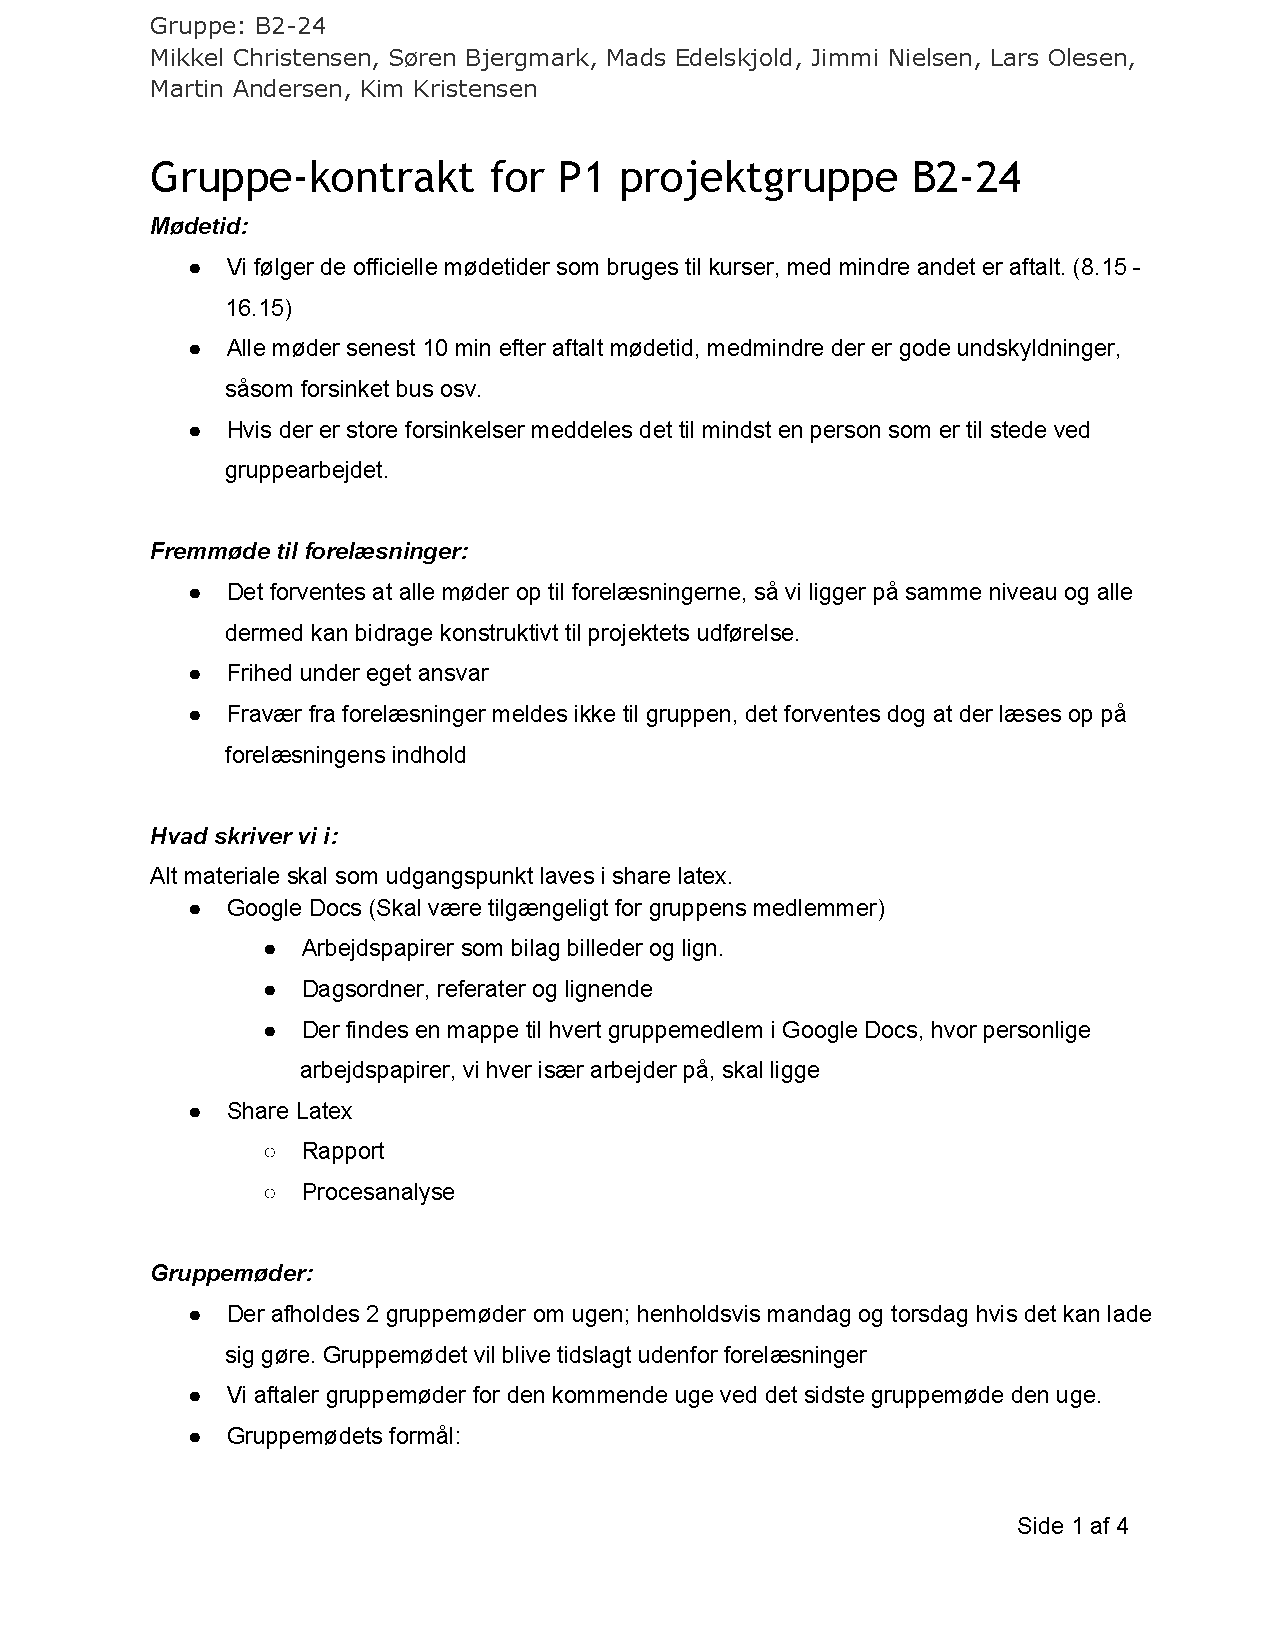
\includepdf[pages=-]{Kapitler/Bilag/gruppekontrakt.pdf}

\subsection{Vejlederkontrakt}
\label{sec:vejlederkontrakt}
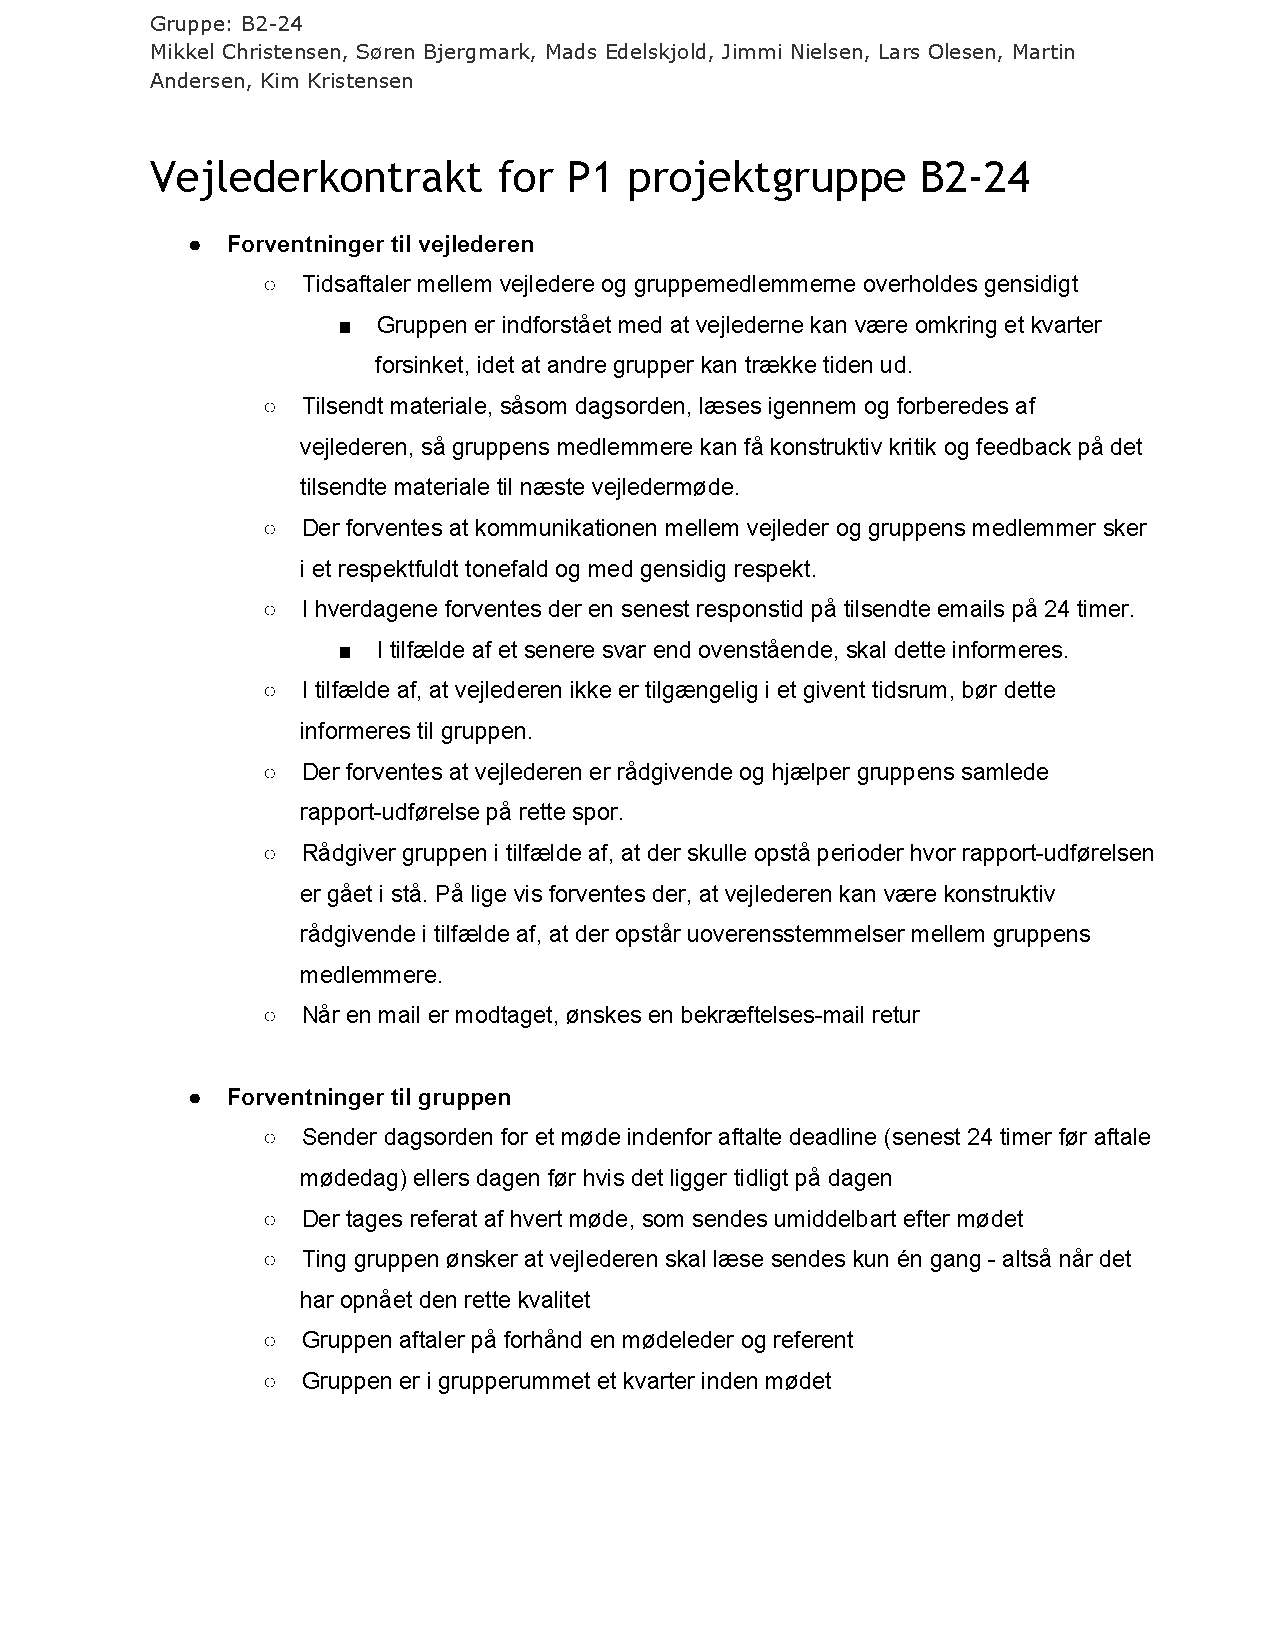
\includepdf[pages=-]{Kapitler/Bilag/Vejlederkontrakt.pdf}

%Note: PDF'erne er indsat i nævnte rækkefølge
%\ref{sec:sporgeskema}

%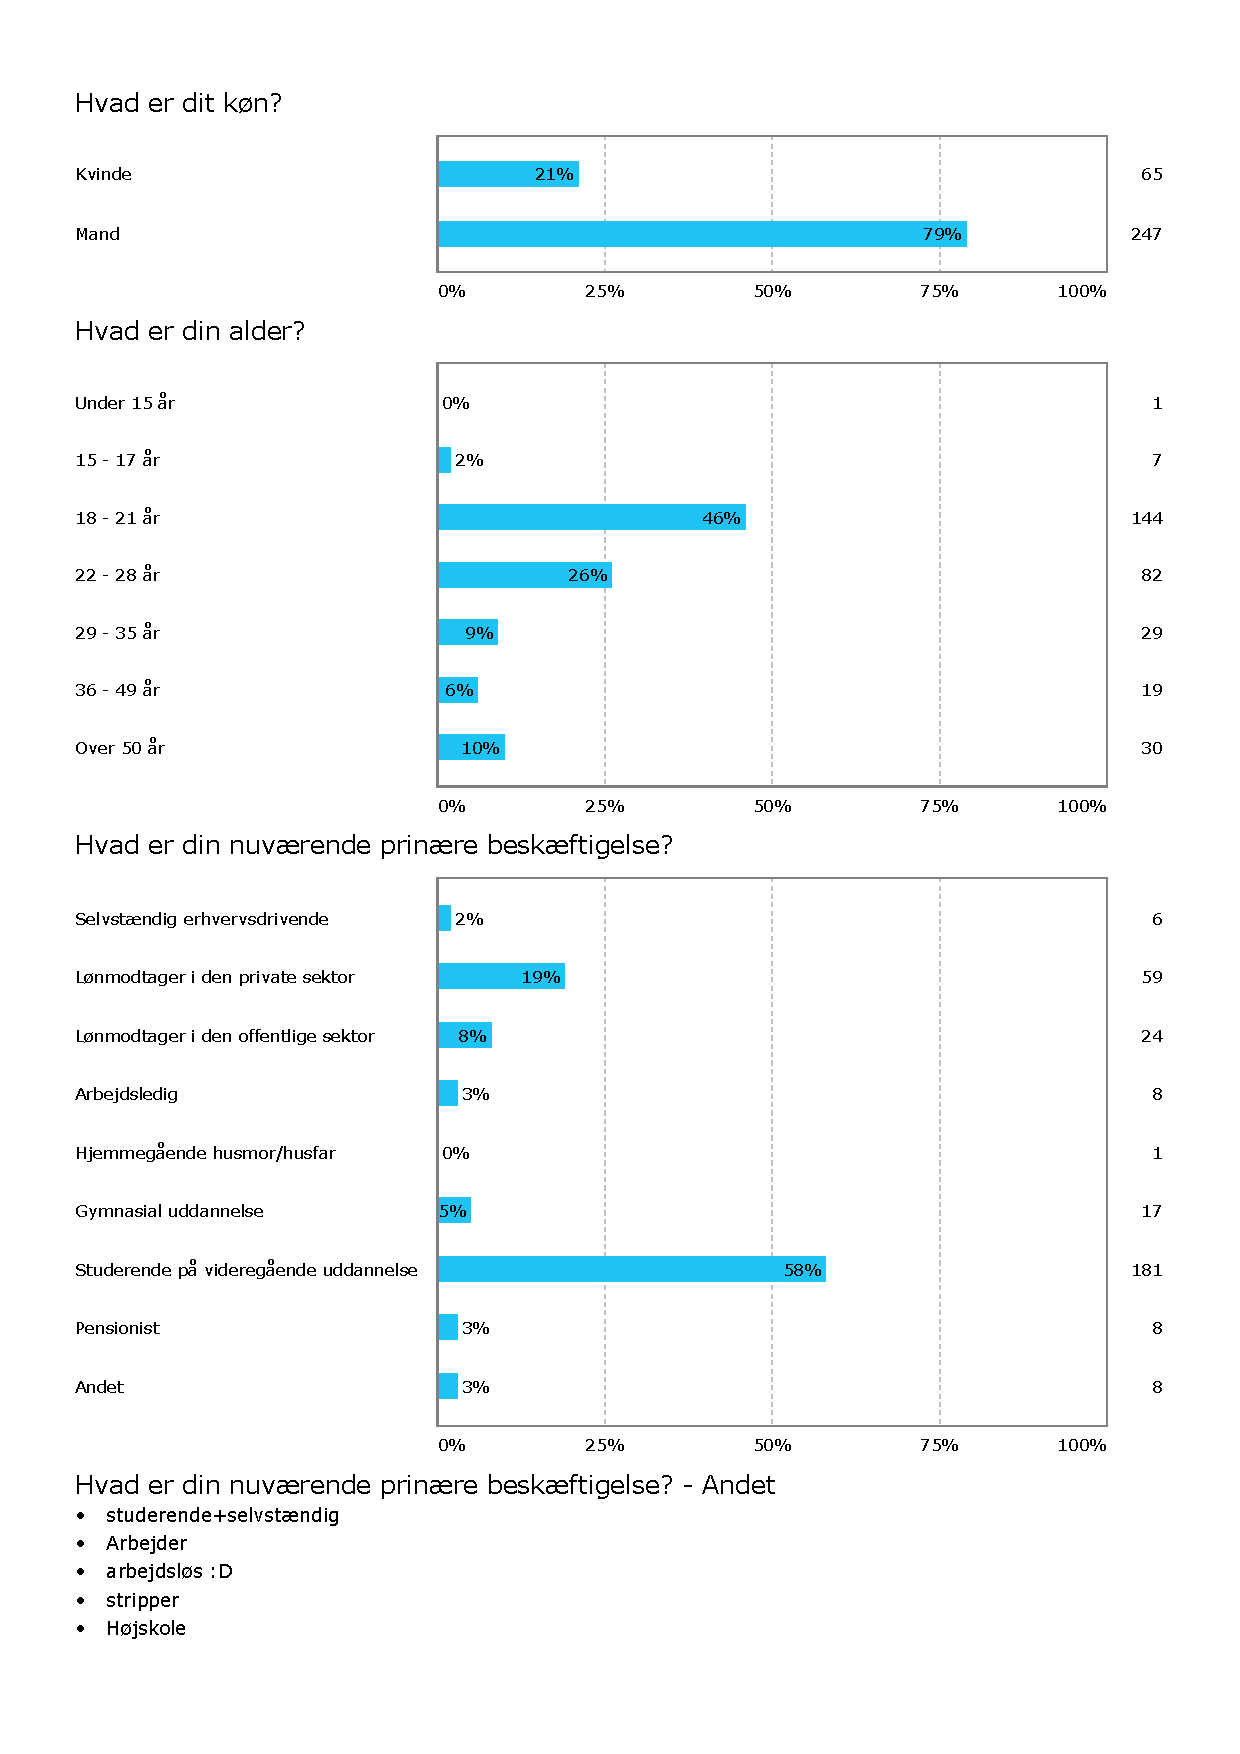
\includepdf[pages=-]{Kapitler/Bilag/Sporgeskema/Alle.pdf}
%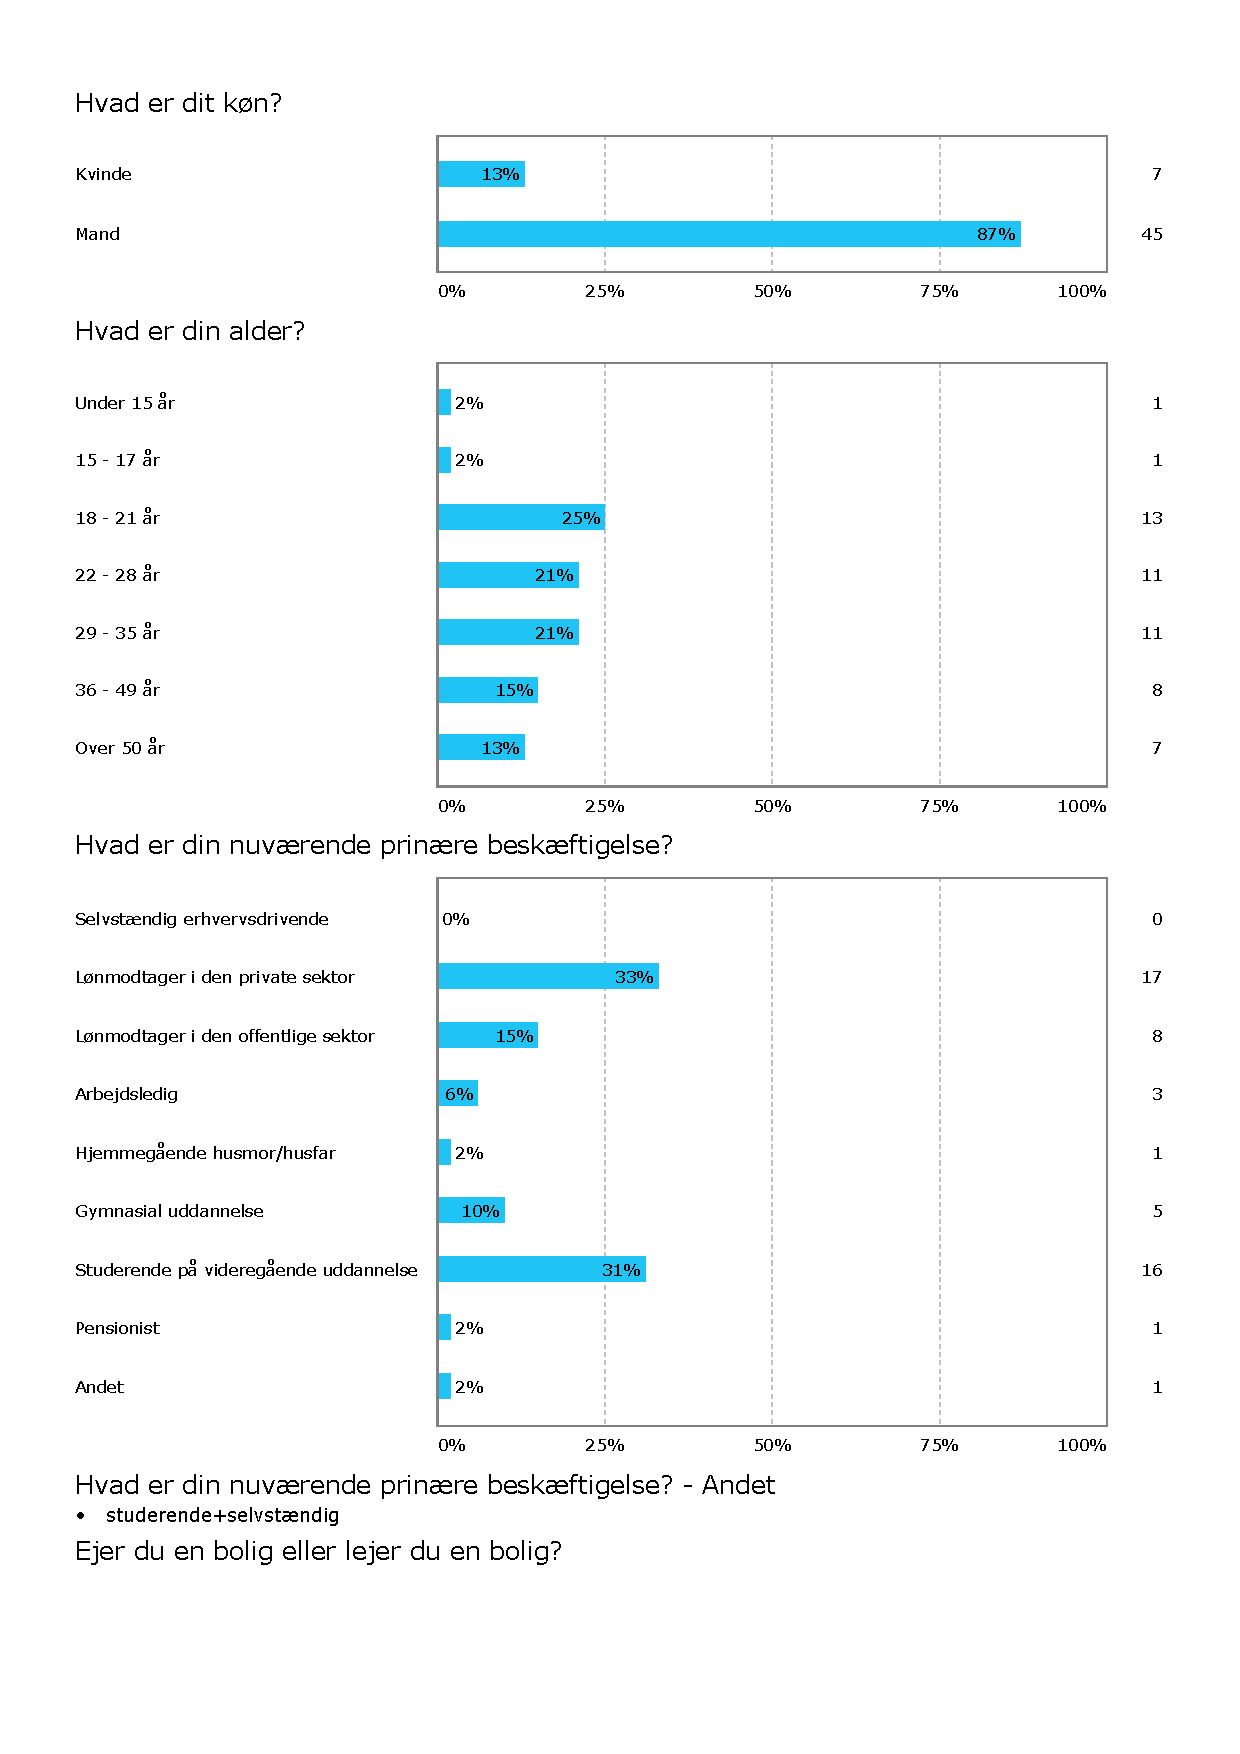
\includepdf[pages=-]{Kapitler/Bilag/Sporgeskema/AutomatiseretHjem.pdf}
%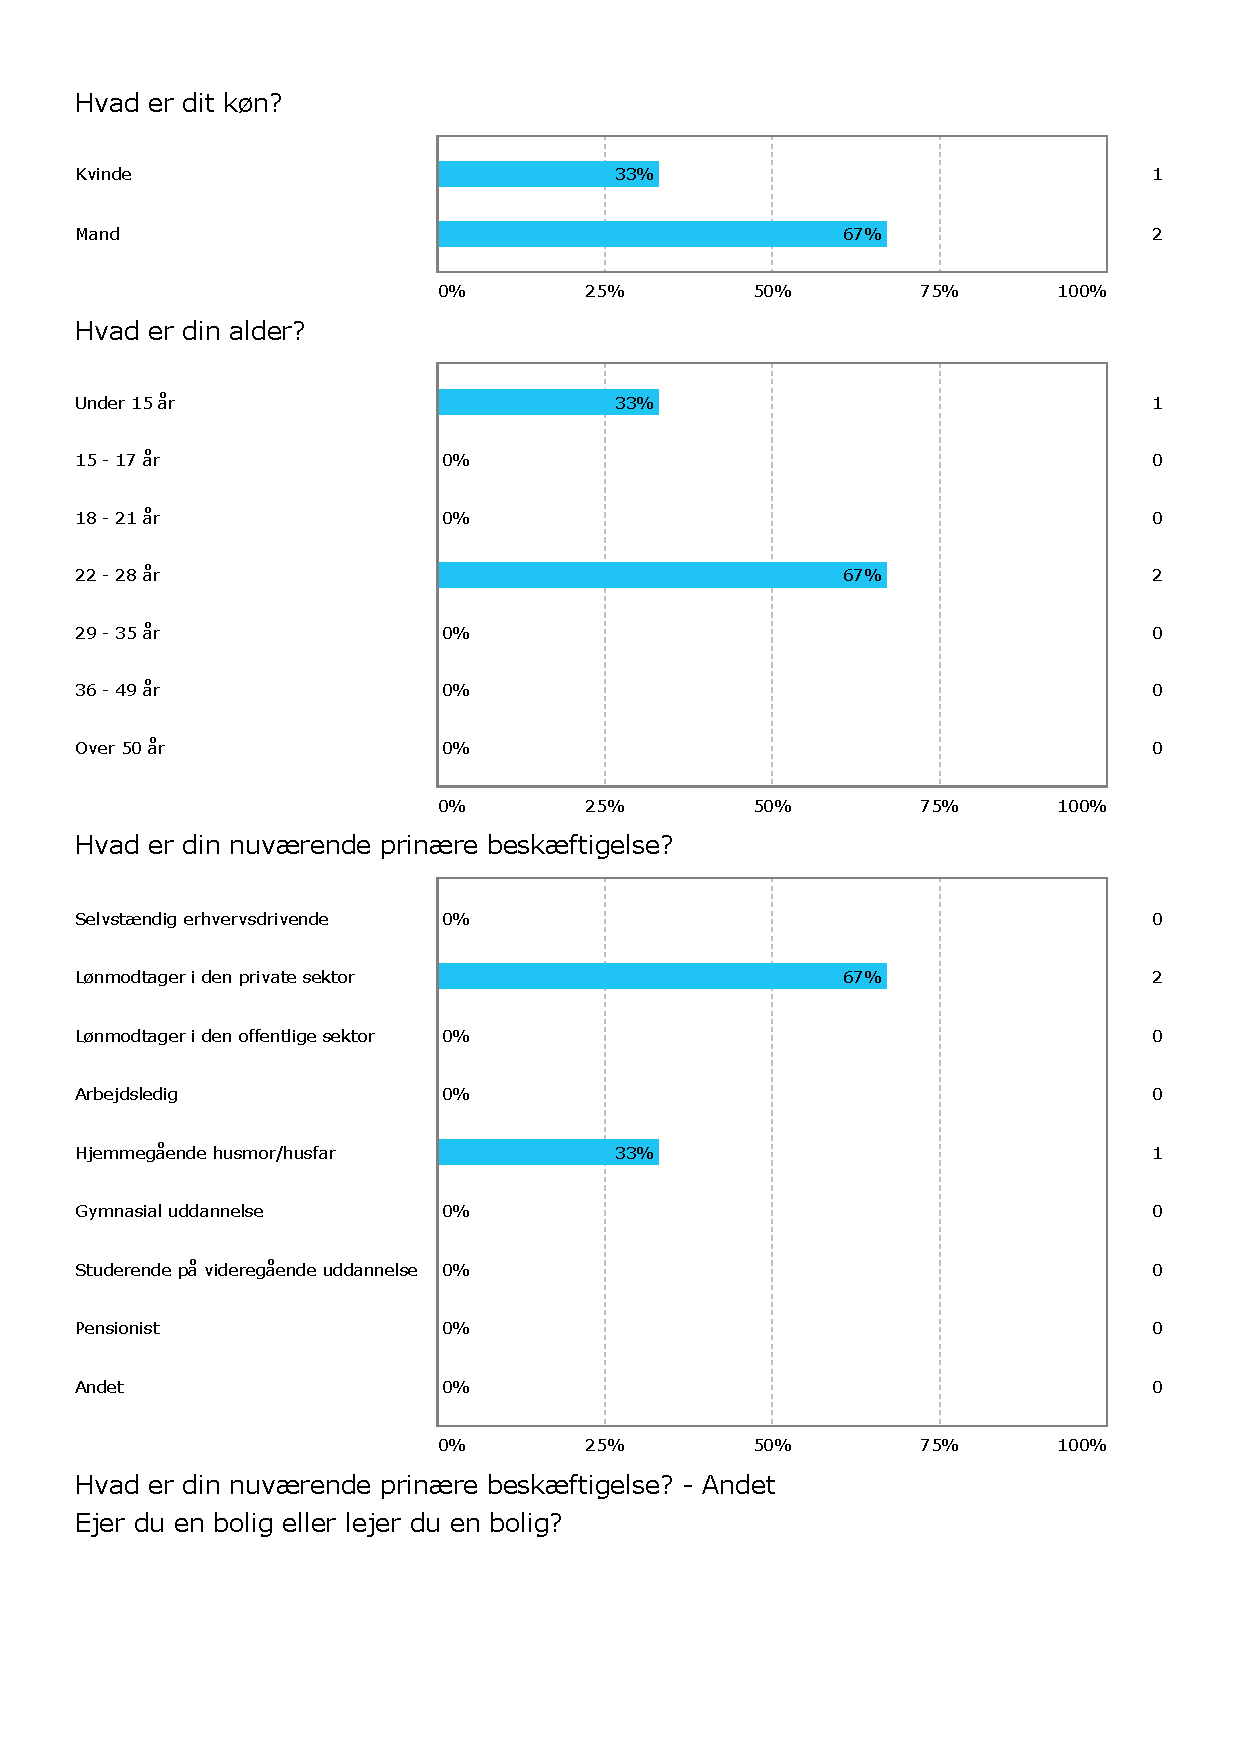
\includepdf[pages=-]{Kapitler/Bilag/Sporgeskema/Zensehome.pdf}
%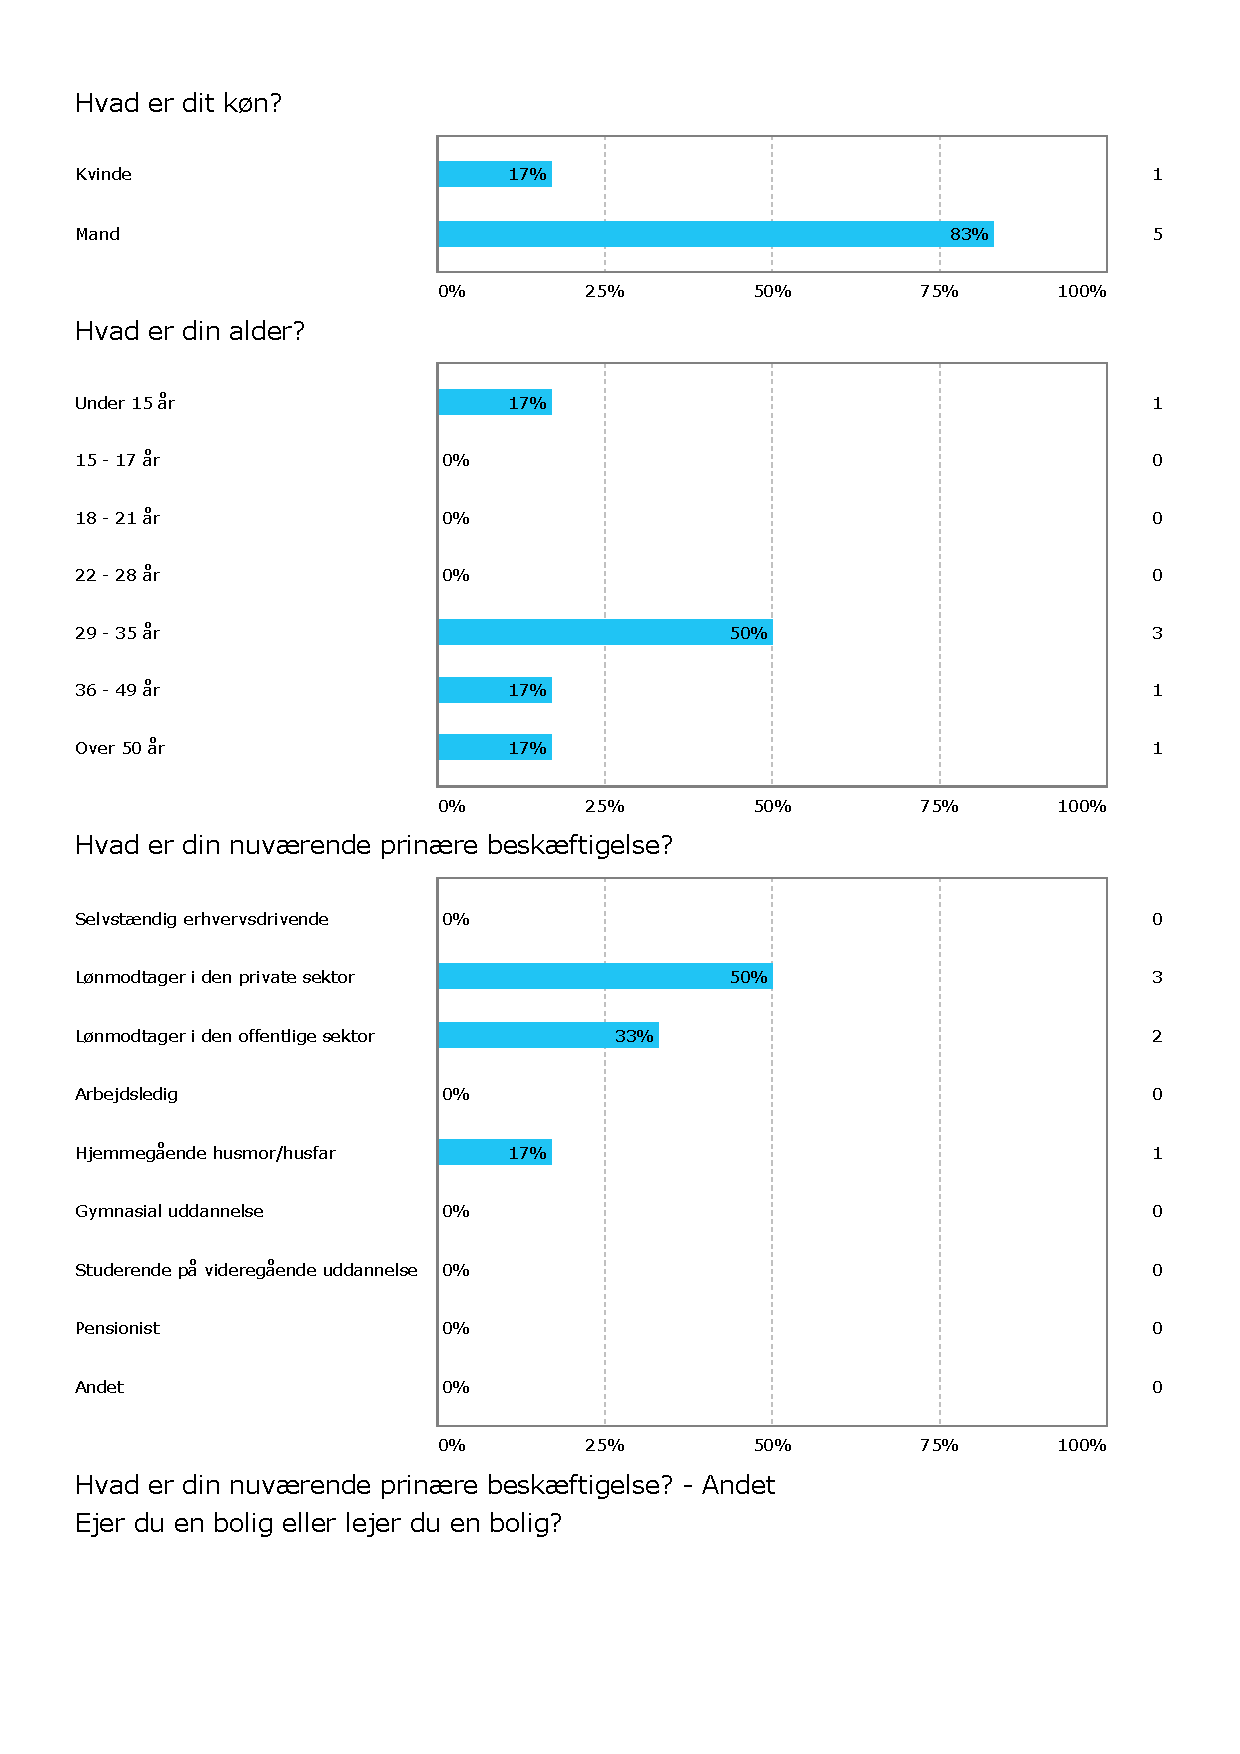
\includepdf[pages=-]{Kapitler/Bilag/Sporgeskema/IHC.pdf}

\end{document}